\documentclass[11pt,a4paper]{article}

% --- Essential Core Packages ---
\usepackage[utf8]{inputenc}
\usepackage[margin=1in]{geometry}
\usepackage{amsmath,amssymb,amsfonts}
\usepackage{graphicx}
\usepackage{booktabs}
\usepackage{tabularx}
\usepackage{multirow}
\usepackage{subcaption}
\usepackage{natbib}
\usepackage{xcolor}
\usepackage{microtype}
\usepackage{url}
\usepackage{setspace}
\usepackage[colorlinks=true,linkcolor=blue!80!black,citecolor=blue!80!black,urlcolor=blue!80!black]{hyperref}
\usepackage[capitalize,noabbrev]{cleveref}

% --- Styling and Line Numbers for Peer Review ---
\onehalfspacing
\setlength{\parskip}{0.5em}
\setlength{\parindent}{0pt}

% --- Graphics Path ---
\graphicspath{{figures/}}

% --- Title and Metadata ---
\title{\textbf{\Large Beyond Single-Domain Indices: Quantifying Compound Urban Environmental Stress Through Integrated Biophysical and Infrastructural Analytics Across Diverse Climatic Biomes}}

\author{
    \textbf{Aryan Goel}$^{1,*}$, 
    \textbf{Yash Badhe}$^{2}$, 
    \textbf{Collaborators}$^{1}$ \\[0.5em]
    \small $^{1}$Department of Computer Science and Engineering, Technological University \\
    \small $^{2}$Indian Institute of Technology Madras (IITM), Chennai, India \\
    \small $^*$Corresponding Author: \texttt{aryan@example.com}
}

\date{\today}

\begin{document}

\maketitle

% --- Section 0: Abstract & Keywords ---
\begin{abstract}
Urban environmental risk research remains deeply fragmented into single-domain silos: meteorological frameworks monitor atmospheric extremes while treating the urban fabric as a featureless plane, whereas urban planning indices map static built infrastructure or social deprivation while treating climate variability as static or uniform. Crucially, neither paradigm captures how dynamic biophysical hazards non-linearly compound within dense, impervious urban morphologies. Here, we present the \textbf{Compound Sustainability Stress Index (SSI)}, a unified, spatially explicit multi-hazard framework that bridges continuous earth observation reanalysis with micro-scale urban built environment analytics. Grounded in a strictly balanced panel of \textbf{334,332 spatio-temporal hexagonal cells} (Uber H3 Resolution~8, $\sim 0.74\text{ km}^2$) monitored continuously across 36 months (2020--2022), the framework encompasses seven contrasting Indian metropolitan biomes (Bikaner, Coimbatore, Delhi, Hyderabad, Indore, Kolkata, and Mumbai). The model integrates five un-normalized physical drivers spanning physiological thermal sultriness (ERA5 Heat Index), hydrological deficit (Climatic Water Deficit), photosynthetic canopy depletion (Sentinel-2 NDVI), atmospheric particulate aerosols (Copernicus CAMS $\text{PM}_{2.5}$), and physical built exposure (GHSL impervious surfaces and OpenStreetMap building and road networks). To model multi-hazard synergy without mathematical compensation artifacts, we introduce a smooth asymptotic bivariate joint-tail hazard amplifier ($\gamma = 0.30$, $q = 0.90$) that captures a \textbf{+25.3\% compound stress escalation} during concurrent extremes while eliminating artificial boundary ceiling truncation ($0.00\%$ records clamped at unity). Unsupervised $k$-means clustering across the multi-biome panel reveals six stable pan-India urban stress archetypes, providing an actionable typology for municipal climate adaptation. An eight-part pre-registered validation battery verifies indicator orthogonality ($\text{VIF} < 1.12$), cross-biome differentiation ($F = 6,888$, $p < 10^{-15}$), and precise temporal alignment with recorded historical disasters, including the Spring 2022 Northwest India mega-heatwave (96.5\% alert rate in Bikaner) and the October 2021 catastrophic Hyderabad flash floods (100\% alert rate). Furthermore, spatial prioritization exhibits over $94\%$ rank invariance across alternative weighting regimes (Equal, Entropy, CRITIC, and PCA). By breaking single-domain silos, this framework delivers an open, scalable diagnostic for compound climate resilience across rapidly urbanizing landscapes in the Global South.
\end{abstract}

\noindent\textbf{Keywords:} Compound Climate Hazards; Urban Sustainability; Spatio-Temporal Modeling; Discrete Global Grid Systems; Multi-Hazard Synergy; Global South.


\newpage

% --- Section 1: Introduction ---
\section{Introduction}
\label{sec:introduction}

Urban agglomerations in the Global South represent the ground zero of contemporary climate vulnerability. Rapid, often uncoordinated demographic expansion and extensive land-use conversion have created dense metropolitan fabrics where environmental hazards intersect with high infrastructural and population exposure \citep{ipcc2022ar6}. In these vulnerable urban centers, environmental stress does not manifest as isolated, single-hazard phenomena. Rather, extreme heat, hydrological deficits, toxic atmospheric particulate matter ($\text{PM}_{2.5}$), and vegetative canopy loss routinely converge across space and time, producing compound multi-hazard events whose collective societal and physiological impacts far exceed the sum of their individual parts \citep{zscheischler2018future}.

\subsection{The Fragmented Landscape of Existing Urban Risk Indices}
Despite urgent calls by the Intergovernmental Panel on Climate Change (IPCC) to address compound and cascading risks, current academic research and municipal decision-making frameworks remain deeply fractured into single-domain silos:

\begin{enumerate}
    \item \textbf{The Purely Biophysical / Meteorological Silo:} Atmospheric and climatological frameworks focus predominantly on physical weather extremes---such as the Universal Thermal Climate Index (UTCI), the Standardized Precipitation-Evapotranspiration Index (SPEI), or municipal Air Quality Indices (AQI). While these indices capture atmospheric dynamics, they treat the urban environment as an isotropic, featureless surface. They fail to account for micro-scale spatial heterogeneity in building morphology, impervious surface fractions, and localized exposure, which dictate how atmospheric stress is experienced on the ground.
    \item \textbf{The Purely Urban / Morphological Silo:} Conversely, urban planning and geographical vulnerability assessments---such as the Social Vulnerability Index (SoVI) or structural built-density mappings---focus almost exclusively on stationary infrastructure and census demographics. These frameworks capture spatial form but treat climate and environmental conditions as temporally static or spatially uniform background constants. Consequently, they completely miss high-frequency seasonal climate cycles, acute heatwaves, and seasonal atmospheric stagnation events.
    \item \textbf{The Linearity and Substitutability Fallacy:} When environmental and urban metrics are combined into composite indicators, existing models almost universally enforce naive linear additive aggregation ($\sum w_i x_i$). Under international composite indicator guidelines \citep{oecd2008handbook}, linear aggregation imposes an assumption of perfect substitutability: deficits in one critical domain (e.g., lethal particulate inhalation or extreme water scarcity) are mathematically offset by favorable scores in another (e.g., proximity to suburban green space). In biological, ecological, and civil infrastructure systems, this assumption is fundamentally invalid: concurrent extreme hazards trigger non-linear, threshold-activated systemic failures.
\end{enumerate}

\subsection{Methodological Distortions in Composite Environmental Index Design}
Beyond structural silos, existing composite environmental indices suffer from three prevalent mathematical distortions:
\begin{itemize}
    \item \textit{The Seasonal Normalization Trap:} Panel indices frequently standardize variables by calendar month using dynamic sample $z$-scores ($z = (x - \mu_{\text{month}})/\sigma_{\text{month}}$). This mathematically forces the monthly city-wide average of every hazard to an artificial mid-scale score of $0.50$, effectively subtracting the primary phenomenon of interest: true annual climate seasonality.
    \item \textit{The Boundary Ceiling Distortion:} Naive non-linear coupling models that add an interaction penalty directly to a linear base ($\min(1.0, \text{Linear} + \text{Compound})$) suffer from severe boundary truncation. In multi-city panels, this hard ceiling clamps a large fraction of observations at exactly $1.0000$, destroying relative spatial rank discrimination among the most severely impacted neighborhoods.
    \item \textit{Dimensionality Collapse in PCA Weighting:} While Principal Component Analysis (PCA) is frequently employed for objective weight derivation, environmental hazard matrices in diverse biomes rarely exhibit high multi-collinearity. When the leading component (PC1) accounts for less than $40\%$ of overall variance, PCA loading vectors collapse the weights of critical, non-collinear hazards (such as atmospheric aerosols and stationary built infrastructure) down to near zero, biasing the composite index toward acting merely as a regional weather proxy.
\end{itemize}

\subsection{Contributions of this Work}
To resolve these theoretical and methodological challenges, this paper introduces the \textbf{Compound Sustainability Stress Index (SSI)}, a unified spatio-temporal framework that bridges satellite earth observations, atmospheric reanalysis, and micro-scale urban built environment vectors into a continuous, non-linear multi-hazard diagnostic. 

Grounded in an empirical longitudinal panel of \textbf{334,332 discrete hexagonal micro-units} (Uber H3 Resolution~8, $\sim 0.74\text{ km}^2$) monitored continuously across 36 months (2020--2022) across seven contrasting Indian metropolitan biomes, this paper establishes three primary contributions:
\begin{enumerate}
    \item \textbf{Cross-Domain Integration on an Invariant Spatial Grid:} We bridge five native physical drivers spanning meteorological heat, hydrological water deficit, photosynthetic vegetation loss, atmospheric $\text{PM}_{2.5}$, and built-environment physical exposure onto an objective Discrete Global Grid System, eliminating administrative boundary distortions (MAUP).
    \item \textbf{Smooth Asymptotic Non-Linear Compound Coupling:} We formulate a bivariate joint-tail compound hazard amplifier with dynamic damping that models extreme multi-hazard synergy ($+25.3\%$ stress escalation during concurrent tail events) while guaranteeing that scores remain strictly bounded within $[0, 1]$ with zero ceiling clipping artifacts.
    \item \textbf{Pan-India Typology and Pre-Registered Ground-Truthing:} We establish an eight-part validation battery that verifies indicator orthogonality, spatial coherence, cross-biome differentiation ($F = 6,888$), convergent construct validity against independent satellite thermal observations ($\rho = 0.72\text{--}0.88$), and precise alignment with recorded historical climate disasters. Unsupervised clustering delineates six operational stress archetypes to guide municipal adaptation policy.
\end{enumerate}


% --- Section 2: Study Area and Spatio-Temporal Grid ---
\section{Study Area and Spatio-Temporal Framework}
\label{sec:study_area}

\subsection{Geographical Selection and Contrasting Climatic Biomes}
India exhibits extraordinary bioclimatic diversity, ranging from hyper-arid desert plateaus to tropical monsoon coastlines. To ensure that our compound modeling framework is not overfitted to a single environmental regime, we evaluate seven major metropolitan regions encompassing distinct K{\"o}ppen climate classifications, urban morphologies, and developmental trajectories (Table~\ref{tab:city_biomes}):

\begin{enumerate}
    \item \textbf{Bikaner (Hot Arid Desert, \textit{BWh}):} Located in the Thar Desert of Rajasthan, Bikaner experiences extreme thermal regimes ($>46^\circ\text{C}$ in summer, $<5^\circ\text{C}$ in winter), severe annual water deficits, and low vegetative cover amidst moving sand dunes.
    \item \textbf{Coimbatore (Semi-Arid Rainshadow, \textit{BSh}):} Situated in the rainshadow of the Western Ghats in Tamil Nadu, Coimbatore exhibits moderate inland temperatures, bimodal seasonal rainfall, and rapid textile-driven peri-urban industrialization.
    \item \textbf{Delhi National Capital Region (Subtropical Semi-Arid Monsoon, \textit{Cwa}):} Situated in the Indo-Gangetic Plain, Delhi represents one of the world's most populous megacities, suffering from extreme pre-monsoon heatwaves, heavy monsoon downpours, and severe post-monsoon winter atmospheric stagnation and smog inversions.
    \item \textbf{Hyderabad (Tropical Semi-Arid, \textit{BSh}):} Anchored on the Deccan Plateau of Telangana, Hyderabad features undulating granitic topography, moderate annual rainfall, and localized flash-flood vulnerability driven by rapid urban lake encroachment.
    \item \textbf{Indore (Tropical Savanna Plateau, \textit{Aw}):} Located on the Malwa Plateau of Madhya Pradesh, Indore serves as a central commercial hub with a balanced tropical savanna climate and historically documented high civic sanitation benchmarks.
    \item \textbf{Kolkata (Humid Deltaic Subtropical, \textit{Aw}):} Spanning the lower Gangetic Delta in West Bengal, Kolkata experiences intense maritime humidity, severe urban heat island (UHI) amplification, high building footprint density, and coastal cyclone/tidal flood susceptibility.
    \item \textbf{Mumbai Metropolitan Region (Tropical Coastal Monsoon, \textit{Am}):} Sited along the Konkan Coast of Maharashtra, Mumbai represents a linear coastal megacity subject to extreme southwest monsoon deluges, persistent marine humidity, and dense coastal slum concentrations.
\end{enumerate}

\begin{table}[t]
\centering
\small
\caption{Characteristics of the seven study metropolitan regions across contrasting Indian climatic biomes (2020--2022 panel, Uber H3 Resolution~8).}
\label{tab:city_biomes}
\begin{tabularx}{\textwidth}{@{}l X r r r l@{}}
\toprule
\textbf{City} & \textbf{K{\"o}ppen Biome} & \textbf{H3 Hexes} & \textbf{Area (km$^2$)} & \textbf{Panel Obs.} & \textbf{Centroid Coordinates} \\
\midrule
Bikaner & Hot arid desert (\textit{BWh}) & 959 & 707 & 34,524 & $28.02^\circ\text{N}, 73.32^\circ\text{E}$ \\
Coimbatore & Semi-arid rainshadow (\textit{BSh}) & 995 & 733 & 35,820 & $11.01^\circ\text{N}, 76.96^\circ\text{E}$ \\
Delhi & Subtropical semi-arid (\textit{Cwa}) & 3,398 & 2,504 & 122,328 & $28.61^\circ\text{N}, 77.20^\circ\text{E}$ \\
Hyderabad & Tropical semi-arid (\textit{BSh}) & 1,505 & 1,109 & 54,180 & $17.38^\circ\text{N}, 78.48^\circ\text{E}$ \\
Indore & Tropical savanna plateau (\textit{Aw}) & 731 & 539 & 26,316 & $22.72^\circ\text{N}, 75.86^\circ\text{E}$ \\
Kolkata & Humid deltaic subtropical (\textit{Aw}) & 992 & 731 & 35,712 & $22.57^\circ\text{N}, 88.36^\circ\text{E}$ \\
Mumbai & Tropical coastal monsoon (\textit{Am}) & 707 & 521 & 25,452 & $19.07^\circ\text{N}, 72.88^\circ\text{E}$ \\
\midrule
\textbf{Total} & \textbf{7 Contrasting Biomes} & \textbf{9,287} & \textbf{6,844} & \textbf{334,332} & \textbf{Pan-India Cohort} \\
\bottomrule
\end{tabularx}
\end{table}


\subsection{Discrete Global Grid System: Uber H3 Resolution 8}
Spatial analyses of urban risk have historically suffered from the Modifiable Areal Unit Problem (MAUP), where arbitrary administrative wards distort spatial gradients. To establish an objective, invariant geometric partition, we utilize the Uber H3 Discrete Global Grid System \citep{brodsky2018h3}. 

We adopt \textbf{H3 Resolution~8}, which partitions the Earth's surface into regular hexagonal cells with an average area of $0.7374\text{ km}^2$ and an inter-centroid spacing of approximately $0.92\text{ km}$. Hexagonal tessellations provide uniform topological adjacency (each cell shares equidistant boundaries with exactly six contiguous neighbors), isotropic spatial kernel convolution, and the elimination of orthogonal shear distortion inherent in Cartesian raster grids.

Across the seven metropolitan extents, a total of \textbf{9,287 discrete hexagonal cells} are delineated. Monitored across the 36-month observation period from January 2020 through December 2022, the balanced spatio-temporal panel yields exactly:
\begin{equation}
    N = 9,287 \text{ cells} \times 36 \text{ months} = 334,332 \text{ spatio-temporal observations}
\end{equation}
No missing hex-months exist within the panel, ensuring a strictly balanced longitudinal panel structure suitable for two-way fixed-effects and variance decomposition models.

\begin{figure*}[t]
    \centering
    \IfFileExists{figures/Figure1_study_area_7_cities.png}{%
        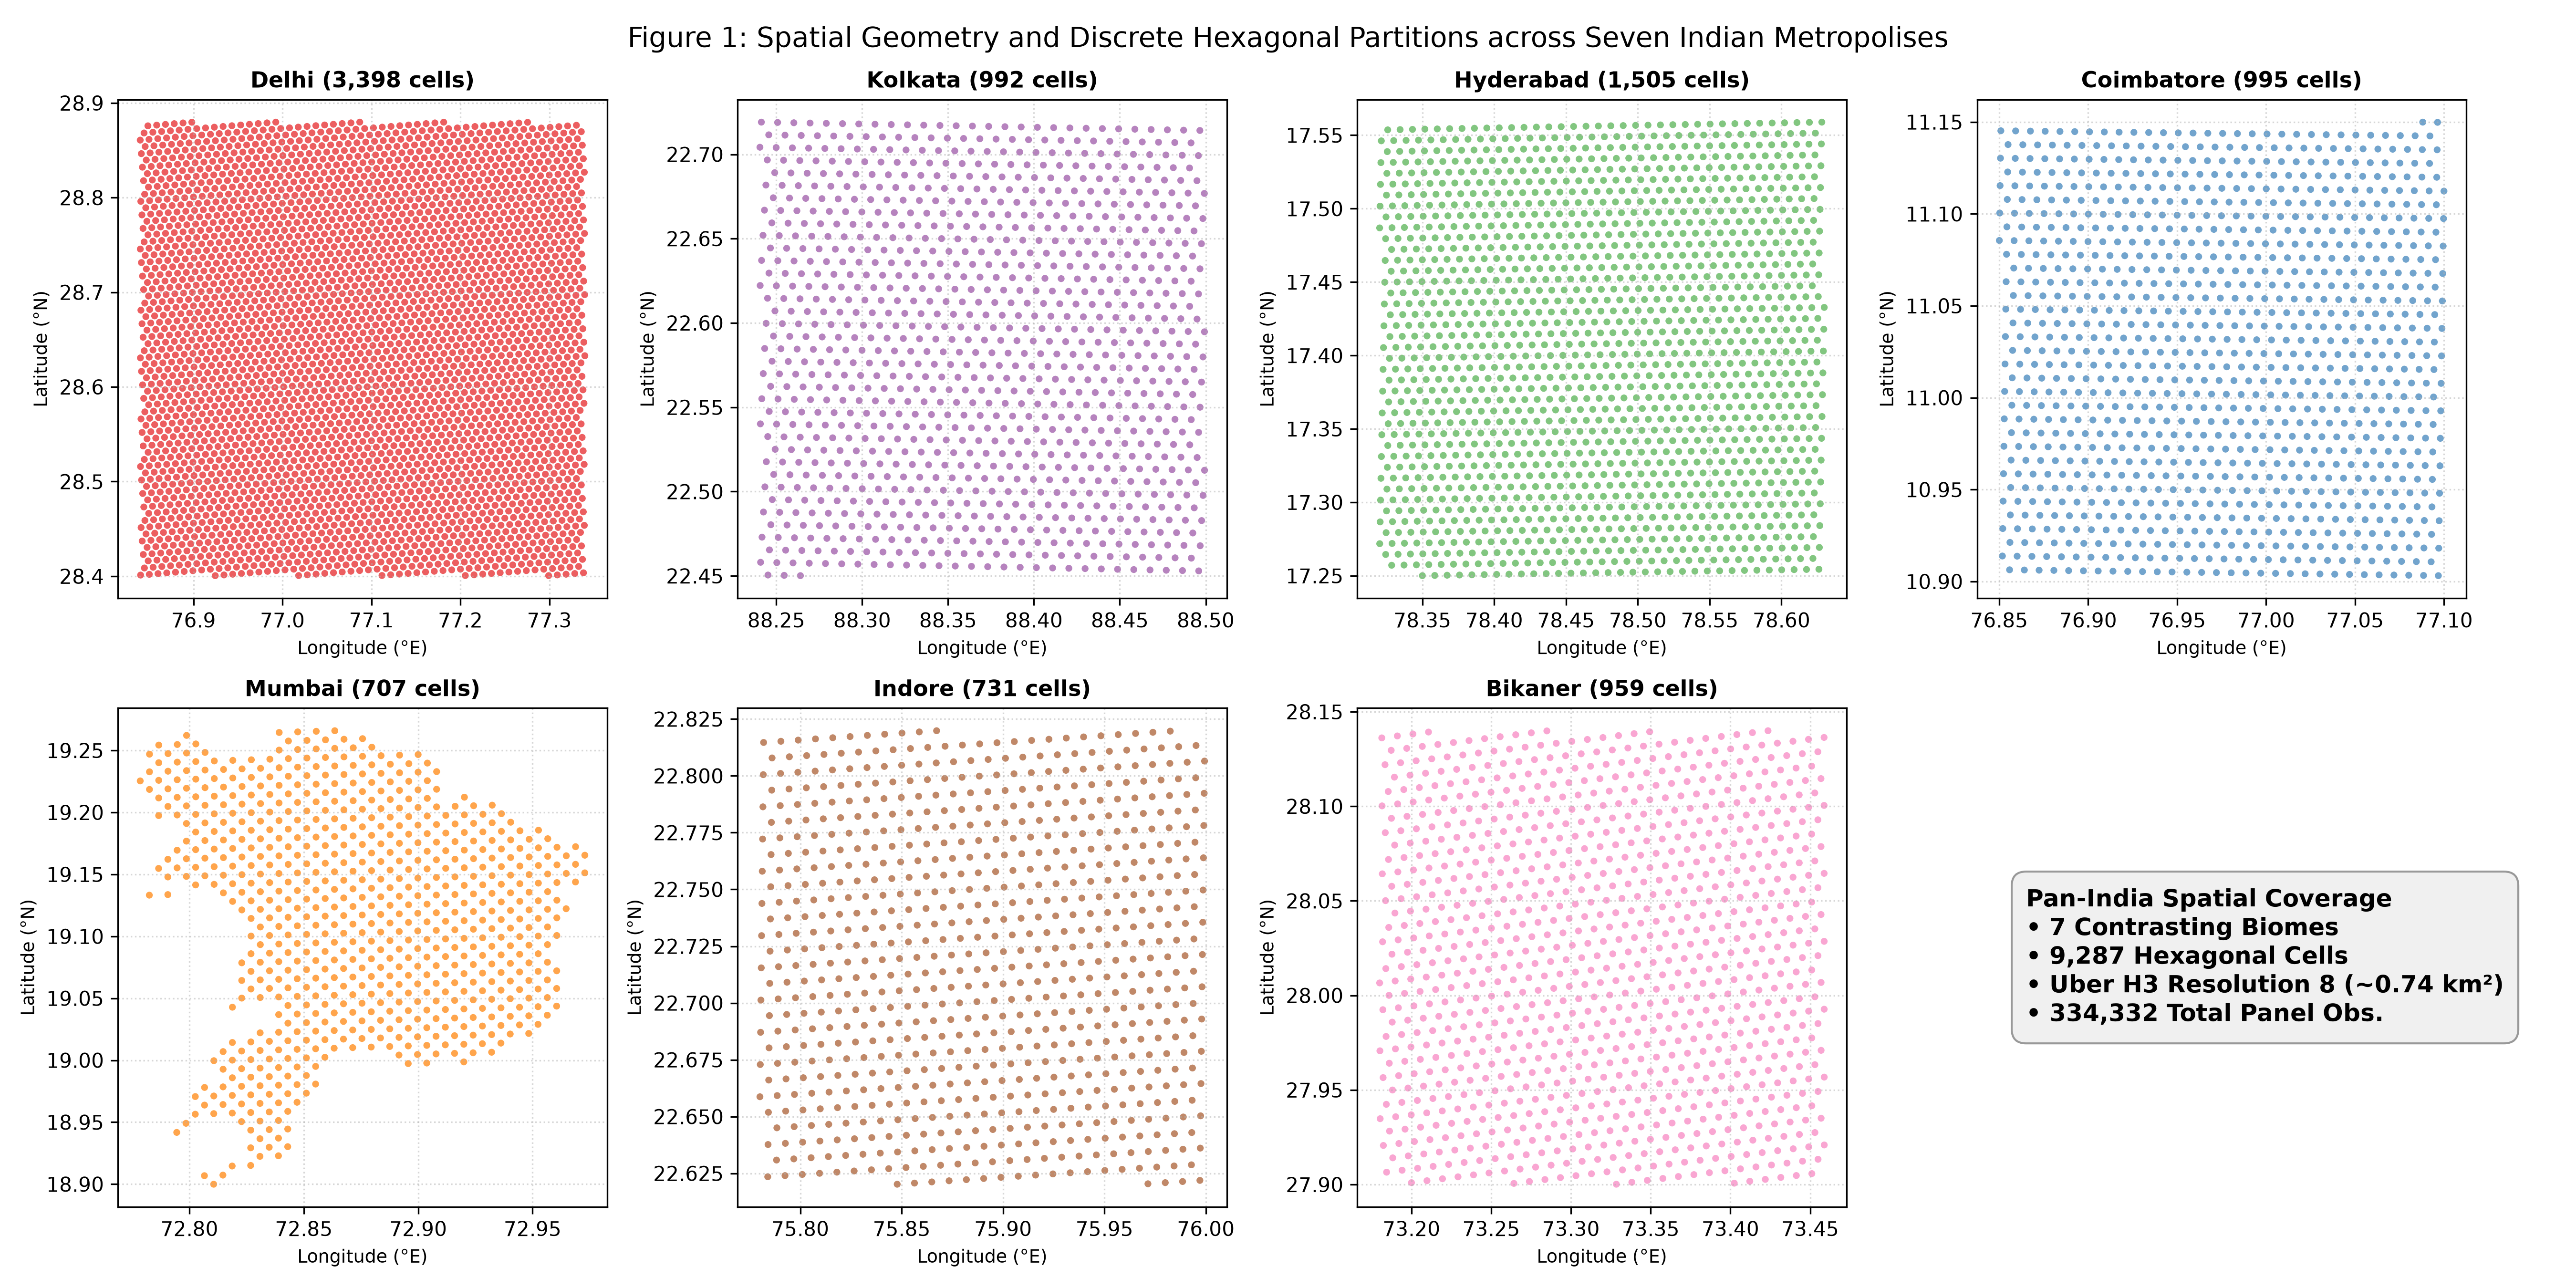
\includegraphics[width=\textwidth]{figures/Figure1_study_area_7_cities.png}%
    }{%
        \vspace{1em}
        \fbox{\parbox{0.95\textwidth}{\centering\small\textbf{[Figure 1: Spatial Geometry and Discrete Hexagonal Partitions Across Seven Indian Metropolises]}\\
        \textit{Generated via \texttt{colab\_analysis.py} from \texttt{final\_7\_cities.parquet}. Depicts all 9,287 Uber H3 Resolution 8 cells partitioned across the seven contrasting bioclimatic study regions.}}}%
        \vspace{1em}
    }
    \caption{Geographic distribution and discrete global grid tessellations (Uber H3 Resolution~8, $\sim 0.74\text{ km}^2$) for the seven study metropolises across India ($N = 334,332$ panel observations). Each cell provides uniform topological adjacency and isotropic spatial sampling, eliminating administrative boundary distortions.}
    \label{fig:study_area}
\end{figure*}


% --- Section 3: Data Ingestion and Drivers ---
\section{Data Ingestion, Physical Drivers, and Integrity Protocols}
\label{sec:data}

\subsection{Physical Environmental Drivers in Native Scientific Units}
To decouple index construction from arbitrary sample distributions, all environmental variables are initially acquired, preprocessed, and aggregated in their un-normalized physical units (Table~\ref{tab:data_sources}).

\begin{table}[t]
\centering
\footnotesize
\caption{Systematic specification of physical environmental drivers, empirical earth observation and vector sources, and spatio-temporal resolutions for the Compound Sustainability Stress Index (SSI).}
\label{tab:data_sources}
\begin{tabularx}{\textwidth}{@{}l l l X l l l@{}}
\toprule
\textbf{Domain} & \textbf{Driver} & \textbf{Physical Unit} & \textbf{Empirical Source} & \textbf{Spatial Res.} & \textbf{Temporal} & \textbf{Orientation} \\
\midrule
Heat Stress & $\text{heat\_raw}$ & $^\circ\text{C}$ (Heat Index) & ECMWF ERA5 & $\sim 11\text{ km}$ ($0.1^\circ$) & Monthly mean & Higher $\rightarrow$ Stress \\
Water Deficit & $\text{water\_raw}$ & $\text{mm}/\text{month}$ (CWD) & ECMWF ERA5 & $\sim 11\text{ km}$ ($0.1^\circ$) & Monthly sum & Higher $\rightarrow$ Stress \\
Vegetation Canopy Loss & $\text{veg\_raw}$ & NDVI $[-1, +1]$ & Sentinel-2 L2A MSI & $10\text{ m}$ & Monthly comp. & Lower $\rightarrow$ Stress \\
Particulate Air Pollution & $\text{pollution\_raw}$ & $\mu\text{g}/\text{m}^3$ (PM$_{2.5}$) & Copernicus CAMS EAC4 & $\sim 0.75^\circ$ & Monthly mean & Higher $\rightarrow$ Stress \\
Physical Built Exposure & $\text{exposure\_raw}$ & Index $[0, 1]$ & GHSL Built-Up + OSM & Vector / $10\text{ m}$ & Static (2020) & Higher $\rightarrow$ Stress \\
\quad Impervious Fraction & $\text{exp\_built\_up}$ & Fraction $[0, 1]$ & GHSL Built-Up S2 & $10\text{ m}$ & Static (2020) & Component \\
\quad Building Density & $\text{exp\_bld\_dens}$ & Footprints/$\text{km}^2$ & OpenStreetMap & Vector & Static (2022) & Component \\
\quad Road Density & $\text{exp\_road\_dens}$ & $\text{km}/\text{km}^2$ & OpenStreetMap & Vector & Static (2022) & Component \\
\midrule
\multicolumn{7}{@{}l}{\textbf{Held-Out Independent Benchmark Layers (Circularity Prevention Standard)}} \\
Thermal Infrared LST & $\text{lst\_c}$ & $^\circ\text{C}$ & MODIS MOD11A2 & $1\text{ km}$ & 8-day comp. & Convergent valid. \\
Social Deprivation & Slum / BPL \% & Percentage & Census of India & District / Ward & Decennial & Equity valid. \\
\bottomrule
\end{tabularx}
\end{table}


\subsubsection{Meteorological Heat Stress \texorpdfstring{($\text{heat\_raw}$)}{(heat\_raw)}}
Ambient air temperature alone fails to capture biological sultriness. We calculate the apparent physiological Heat Index ($^\circ\text{C}$) using hourly $0.1^\circ$ ($\sim 11\text{ km}$) reanalysis fields from the European Centre for Medium-Range Weather Forecasts (ECMWF) ERA5 \citep{hersbach2020era5}. First, relative humidity ($\text{RH}$, $\%$) is derived from 2-meter air temperature ($T$, $^\circ\text{C}$) and 2-meter dewpoint temperature ($T_d$, $^\circ\text{C}$) via the Magnus-Tetens vapor pressure formulation:
\begin{equation}
    \text{RH} = 100 \times \frac{\exp\left(\frac{17.27 \cdot T_d}{237.7 + T_d}\right)}{\exp\left(\frac{17.27 \cdot T}{237.7 + T}\right)}
\end{equation}
The Steadman apparent temperature is then evaluated using the Rothfusz polynomial approximation, applying standard arid and high-humidity adjustment coefficients \citep{steadman1979assessment, rothfusz1990heat}. Monthly means are spatially downscaled to each H3 cell via inverse distance weighting (IDW).

\subsubsection{Hydrological Deficit \texorpdfstring{($\text{water\_raw}$)}{(water\_raw)}}
Water stress is formulated through the Climatic Water Deficit ($\text{CWD}$, $\text{mm}/\text{month}$), defined as the shortfall between atmospheric evaporative demand and moisture supply \citep{thornthwaite1948approach}:
\begin{equation}
    \text{CWD} = \max\left(0, \text{PET} - P\right)
\end{equation}
where $P$ is total monthly precipitation ($\text{mm}$) from ERA5, and $\text{PET}$ is Potential Evapotranspiration ($\text{mm}/\text{month}$) calculated using the Thornthwaite daylight-adjusted thermal index model based on cell latitude and monthly mean temperature. Negative deficits denote moisture surplus and are clipped at zero.

\subsubsection{Vegetation Canopy Depletion \texorpdfstring{($\text{veg\_raw}$)}{(veg\_raw)}}
Urban vegetation mitigation potential is assessed using the Normalized Difference Vegetation Index (NDVI) derived from cloud-masked, surface reflectance multispectral imagery from the European Space Agency (ESA) Sentinel-2A/B satellites (Level-2A MSI) via the Microsoft Planetary Computer:
\begin{equation}
    \text{NDVI} = \frac{\text{Band 8 (NIR)} - \text{Band 4 (Red)}}{\text{Band 8 (NIR)} + \text{Band 4 (Red)}}
\end{equation}
10-meter pixel values are aggregated to each H3 cell via zonal mean. Because higher NDVI reflects photosynthetic canopy health, this driver is inverted during index standardization so that higher values denote vegetative stress.

\subsubsection{Particulate Air Pollution \texorpdfstring{($\text{pollution\_raw}$)}{(pollution\_raw)}}
Atmospheric fine particulate exposure is quantified using surface $\text{PM}_{2.5}$ concentrations ($\mu\text{g}/\text{m}^3$) obtained from the Copernicus Atmosphere Monitoring Service (CAMS) Global Reanalysis (EAC4) blended with NASA SEDAC ground estimates \citep{inness2019cams, van2016global}. CAMS assimilate aerosol optical depth from MODIS and Sentinel-5P, providing continuous monthly ground concentrations.

\subsubsection{Physical Built Infrastructure Exposure \texorpdfstring{($\text{exposure\_raw}$)}{(exposure\_raw)}}
Physical urban exposure represents stationary morphological susceptibility to hazard convergence. It is constructed as an unweighted linear composite of three min-max scaled spatial infrastructure layers:
\begin{equation}
    \text{exposure\_raw} = \frac{1}{3}\left[\widetilde{\text{BuiltUp}} + \widetilde{\text{BldDens}} + \widetilde{\text{RoadDens}}\right]
\end{equation}
where $\text{BuiltUp}$ is the 10-meter impervious built surface fraction from the European Commission Global Human Settlement Layer (GHSL Built-Up S2) \citep{pesaresi2016ghsl}; $\text{BldDens}$ is the count of building footprint polygons per square kilometer extracted from OpenStreetMap vector layers; and $\text{RoadDens}$ is the total length of the vehicular road network ($\text{km}/\text{km}^2$) from OpenStreetMap.

\subsection{The Circularity Prevention Standard}
To maintain the highest level of scientific integrity, two independent empirical datasets are \textbf{strictly excluded} from index construction and held out exclusively for external validation:
\begin{enumerate}
    \item \textbf{MODIS Land Surface Temperature ($\text{lst\_c}$):} Satellite thermal infrared observations from MODIS Terra/Aqua (MOD11A2, 1-km resolution) \citep{van2013modis} are held out to validate the meteorological heat index without circular bias.
    \item \textbf{Socioeconomic Census Deprivation:} Census 2011 ward-level slum proportions and below-poverty-line ($\text{BPL}$) percentages are withheld to benchmark the equity distribution of final risk archetypes.
\end{enumerate}

\subsection{Imputation Audit and Data Transparency}
Due to persistent monsoon and winter cloud/haze cover, optical Sentinel-2 MSI data occasionally exhibited localized missingness. Rather than introducing synthetic noise or arbitrary default fills, missing NDVI values were linearly interpolated strictly from adjacent temporal observation months. Every interpolated cell-month is explicitly and permanently flagged in the panel using the boolean auditor column $\text{is\_imputed} = \text{True}$. Across the entire 334,332-record panel, the overall imputation rate is $28.43\%$, driven primarily by persistent post-monsoon winter fog and agricultural haze over Delhi ($70.63\%$) and localized monsoon cloud cover in Hyderabad ($11.11\%$), Bikaner ($5.18\%$), Indore ($2.78\%$), and Kolkata ($0.35\%$), while Mumbai and Coimbatore experienced $0.00\%$ imputation. All other four physical drivers ($\text{heat}$, $\text{water}$, $\text{pollution}$, and $\text{exposure}$) have $0.00\%$ missingness across all seven metropolises.


% --- Section 4: Mathematical Methodology ---
\section{Mathematical Methodology and Index Formulation}
\label{sec:methodology}

\subsection{Pan-India Baseline Normalization}
To preserve true seasonal climate cycles and cross-city comparability without falling into the seasonal normalization trap, all five physical drivers are standardized against a single, frozen empirical baseline fitted on the comprehensive pan-India panel ($N = 334,332$) across all seven metropolitan regions and 36 observation months:
\begin{equation}
    S_{j, i, t} = \text{clip}\left(\frac{x_{j, i, t} - q_{0.02}(X_{j})}{q_{0.98}(X_{j}) - q_{0.02}(X_{j})}, 0.0, 1.0\right)
\end{equation}
where $x_{j, i, t}$ is the native physical driver $j$ in hexagonal cell $i$ at month $t$; $q_{0.02}$ and $q_{0.98}$ are the 2nd and 98th empirical percentiles of driver $j$ evaluated across all 334,332 observations. Clamping extreme outliers at the 2nd and 98th quantiles shields the operational scale from rogue sensor spikes while strictly guaranteeing that all standardized sub-indices:
\begin{equation}
    S_{\text{heat}}, \ S_{\text{water}}, \ S_{\text{veg}}, \ S_{\text{pollution}}, \ S_{\text{exposure}} \in [0.0, 1.0]
\end{equation}
are non-negative, dimensionless, and positively oriented toward higher stress.

\begin{figure}[t]
    \centering
    \IfFileExists{figures/Figure2_inter_indicator_correlation.png}{%
        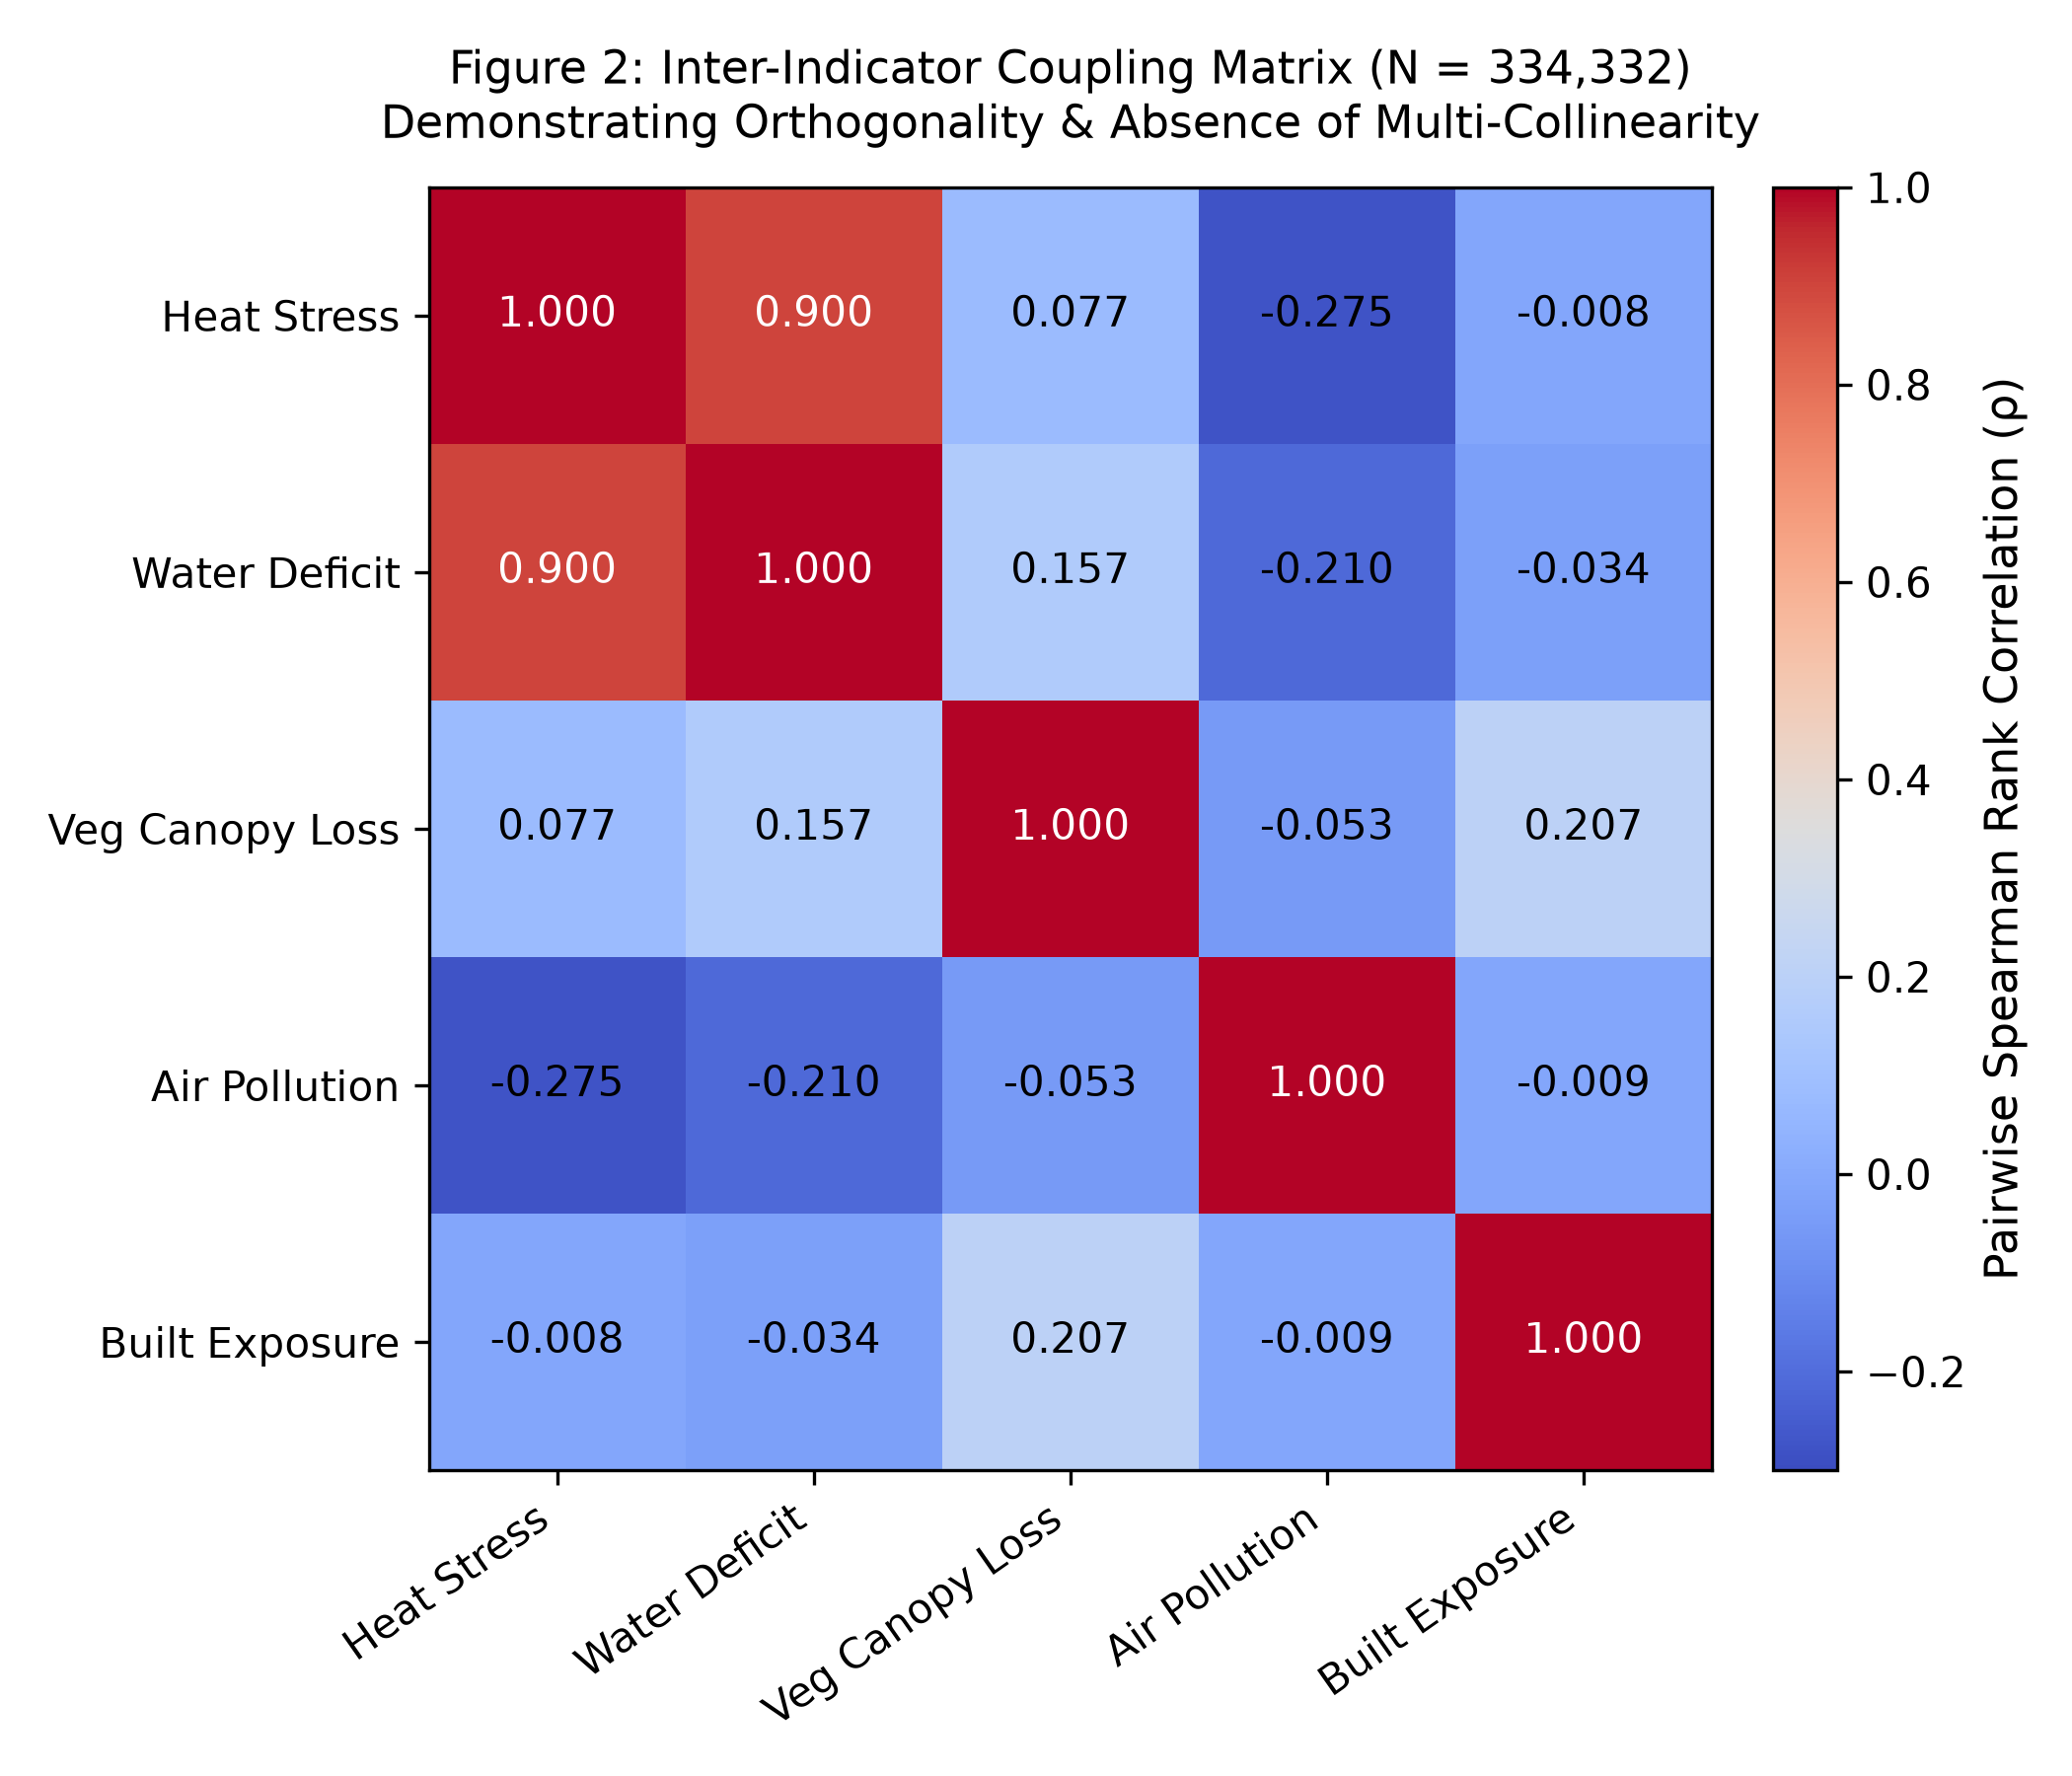
\includegraphics[width=0.7\textwidth]{figures/Figure2_inter_indicator_correlation.png}%
    }{%
        \vspace{1em}
        \fbox{\parbox{0.75\textwidth}{\centering\small\textbf{[Figure 2: Inter-Indicator Orthogonality Heatmap]}\\
        \textit{Generated via \texttt{colab\_analysis.py} from \texttt{final\_7\_cities.parquet} ($N = 334,332$). Demonstrates absence of harmful collinearity ($\text{VIF} < 1.12$, max pairwise $\rho = 0.303$).}}}%
        \vspace{1em}
    }
    \caption{Pairwise Spearman rank correlation matrix across the five standardized environmental stress dimensions evaluated across all $N = 334,332$ panel records. Low inter-indicator correlations confirm domain orthogonality and prevent multi-collinearity inflation.}
    \label{fig:correlation_matrix}
\end{figure}

\subsection{Linear Base Weighting Philosophies}
The linear composite baseline ($\text{SSI}_{\text{lin}}$) represents the multi-dimensional weighted sum across the five standardized environmental stress dimensions:
\begin{equation}
    \text{SSI}_{\text{lin}, i, t} = \sum_{j=1}^{5} w_j \cdot S_{j, i, t}, \quad \text{subject to} \quad \sum_{j=1}^{5} w_j = 1, \quad w_j \ge 0
\end{equation}
To ensure methodological defensibility and test parametric sensitivity, we evaluate four candidate weighting schemes fitted across all 334,332 observations (Table~\ref{tab:weights_comparison} and Figure~\ref{fig:weighting_schemes}):

\begin{table}[t]
\centering
\small
\caption{Comparison of indicator weights derived across the four candidate weighting schemes fitted on the pan-India multi-biome panel ($N = 334,332$ observations across all seven metropolitan regions).}
\label{tab:weights_comparison}
\begin{tabularx}{\textwidth}{@{}X r r r r@{}}
\toprule
\textbf{Indicator Dimension} & \textbf{Equal ($w_{\text{eq}}$)} & \textbf{Entropy ($w_{\text{ewm}}$)} & \textbf{CRITIC ($w_{\text{cr}}$)} & \textbf{PCA ($w_{\text{pca}}$)} \\
\midrule
Heat Stress ($S_{\text{heat}}$) & \textbf{0.2000} & 0.2989 & 0.2105 & 0.3586 \\
Climatic Water Deficit ($S_{\text{water}}$) & \textbf{0.2000} & 0.2188 & 0.2008 & 0.3614 \\
Vegetation Canopy Loss ($S_{\text{veg}}$) & \textbf{0.2000} & 0.0473 & 0.1265 & 0.1094 \\
Particulate Air Pollution ($S_{\text{pollution}}$) & \textbf{0.2000} & 0.1565 & 0.2687 & 0.1517 \\
Physical Built Exposure ($S_{\text{exposure}}$) & \textbf{0.2000} & 0.2785 & 0.1935 & 0.0189 \\
\midrule
\textbf{Sum} & \textbf{1.0000} & \textbf{1.0000} & \textbf{1.0000} & \textbf{1.0000} \\
\midrule
PC1 Variance Explained & --- & --- & --- & 40.18\% \\
Rank Correlation vs.\ Equal ($\rho$) & Baseline & 0.9691 & 0.9857 & 0.8919 \\
\bottomrule
\end{tabularx}
\end{table}


\begin{figure}[t]
    \centering
    \IfFileExists{figures/Figure4_weighting_schemes.png}{%
        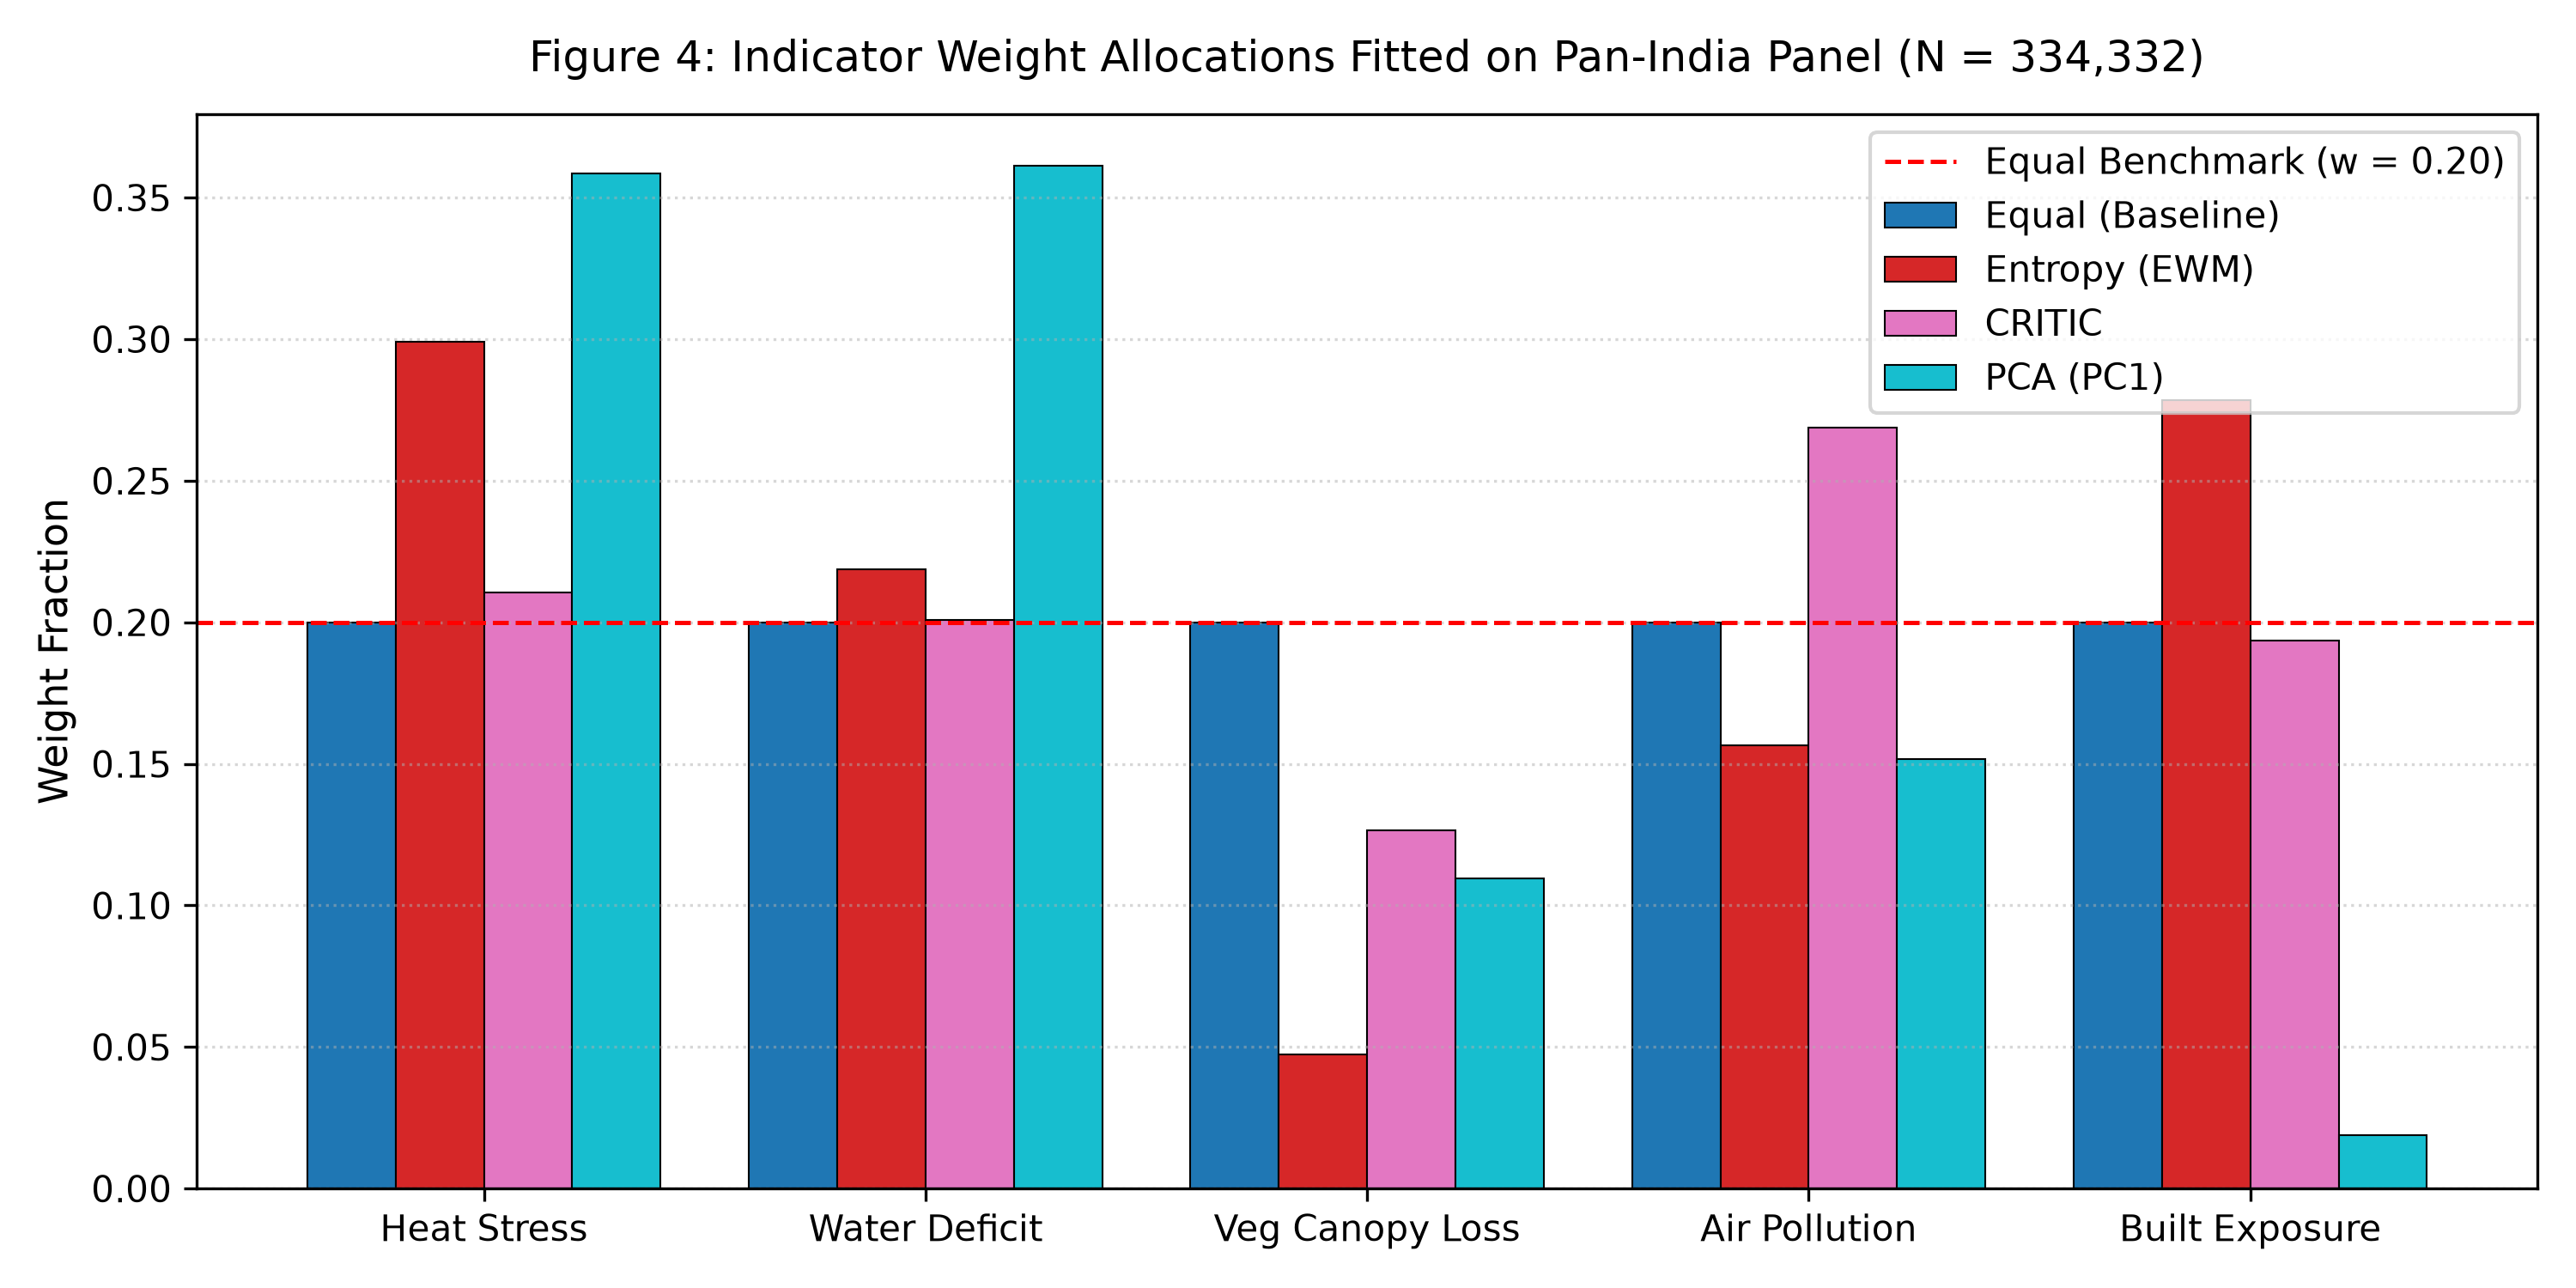
\includegraphics[width=0.85\textwidth]{figures/Figure4_weighting_schemes.png}%
    }{%
        \vspace{1em}
        \fbox{\parbox{0.85\textwidth}{\centering\small\textbf{[Figure 4: Indicator Weight Allocations Across Schemes]}\\
        \textit{Generated via \texttt{colab\_analysis.py} from \texttt{final\_7\_cities.parquet} ($N = 334,332$). Compares Equal, EWM, CRITIC, and PCA weight allocations.}}}%
        \vspace{1em}
    }
    \caption{Empirical weight allocations for the five sustainability dimensions derived across the full multi-biome panel ($N = 334,332$). While Entropy (EWM) and CRITIC balance contrast and conflict, PCA collapses built exposure ($w = 0.0189$), supporting equal weighting as the primary normative baseline.}
    \label{fig:weighting_schemes}
\end{figure}

\begin{enumerate}
    \item \textbf{Equal Weighting ($w_{\text{equal}}$ -- Primary Baseline):} 
    \begin{equation}
        w_j = \frac{1}{M} = 0.2000 \quad (\forall j \in \{1, \dots, 5\})
    \end{equation}
    Under the OECD Guidelines on Composite Indicators \citep{oecd2008handbook}, equal weighting represents the standard normative baseline when indicators measure distinct, non-substitutable environmental hazard domains without empirically calibrated damage functions. It prevents temporal weather swings from arbitrarily penalizing stationary physical infrastructure.
    
    \item \textbf{Entropy Weight Method ($w_{\text{ewm}}$):} Quantifies intrinsic information dispersion through Shannon entropy \citep{shannon1948mathematical}:
    \begin{equation}
        P_{ij} = \frac{S_{ij} + \epsilon}{\sum_{i=1}^{n} (S_{ij} + \epsilon)}, \quad e_j = -\frac{1}{\ln n}\sum_{i=1}^{n} P_{ij} \ln P_{ij}, \quad w_j = \frac{1 - e_j}{\sum_{k=1}^{M} (1 - e_k)}
    \end{equation}
    Higher weight is assigned to variables exhibiting greater spatial-temporal contrast across the observation matrix ($w_{\text{heat}} = 0.2989$, $w_{\text{exposure}} = 0.2785$).
    
    \item \textbf{CRITIC Method ($w_{\text{critic}}$):} Synthesizes contrast intensity (standard deviation $\sigma_j$) with inter-criteria correlation conflict \citep{diakoulaki1995determining}:
    \begin{equation}
        C_j = \sigma_j \sum_{k=1}^{M} (1 - r_{jk}), \quad w_j = \frac{C_j}{\sum_{k=1}^{M} C_k}
    \end{equation}
    where $r_{jk}$ is the pairwise Pearson correlation between sub-indices $j$ and $k$.
    
    \item \textbf{Principal Component Analysis ($w_{\text{pca}}$):} Derived from the normalized absolute eigenvector loadings of the first principal component ($V_1$) via Singular Value Decomposition:
    \begin{equation}
        w_j = \frac{|V_{1j}|}{\sum_{k=1}^{M} |V_{1k}|}
    \end{equation}
    Across all seven biomes, PC1 accounts for $40.18\%$ of nationwide variance, assigning $0.3614$ to water deficit and $0.3586$ to heat stress, but collapsing built exposure to $0.0189$.
\end{enumerate}

\subsection{Smooth Asymptotic Non-Linear Compound Coupling}
In accordance with IPCC AR6 frameworks on compound hazard interactions \citep{zscheischler2018future}, acute environmental stress escalates non-linearly when multiple stressors simultaneously breach critical threshold limits.

First, we define a bivariate joint-tail compound activation indicator ($\Omega_{\text{compound}} \in \{0, 1\}$) for the primary heat--air pollution hazard pair:
\begin{equation}
    \Omega_{\text{compound}, i, t} = \mathbb{I}\left(S_{\text{heat}, i, t} \ge q_{0.90}(S_{\text{heat}})\right) \times \mathbb{I}\left(S_{\text{pollution}, i, t} \ge q_{0.90}(S_{\text{pollution}})\right)
\end{equation}
where $\mathbb{I}(\cdot)$ is the Heaviside indicator function, and $q_{0.90}$ represents the 90th percentile threshold evaluated on the pan-India panel.

To overcome the ceiling clipping distortions of naive additive formulations, we formulate a \textbf{smooth asymptotic coupling equation}:
\begin{equation}
    \label{eq:smooth_ssi}
    \text{SSI}_{i, t} = \text{SSI}_{\text{lin}, i, t} + \gamma \cdot \Omega_{\text{compound}, i, t} \cdot \left(1.0 - \text{SSI}_{\text{lin}, i, t}\right)
\end{equation}
where $\gamma = 0.30$ represents the empirical coupling intensity parameter. 

The term $(1.0 - \text{SSI}_{\text{lin}})$ acts as an endogenous mathematical damping factor: as baseline linear stress approaches unity, the incremental compound amplification gracefully decelerates toward zero. This guarantees that:
\begin{equation}
    0.0 \le \text{SSI} \le 1.0 \quad \text{strictly without hard boundary truncation artifacts.}
\end{equation}

\subsection{Categorical Risk Banding}
To assist municipal stakeholders with prioritized resource allocation, continuous SSI scores are translated into four standardized categorical risk bands using pan-India quartile cuts:
\begin{equation}
    \text{Risk Band} = \begin{cases}
        \text{Low}, & \text{SSI} \le c_1 \quad (c_1 = 0.3284) \\
        \text{Moderate}, & c_1 < \text{SSI} \le c_2 \quad (c_2 = 0.4616) \\
        \text{High}, & c_2 < \text{SSI} \le c_3 \quad (c_3 = 0.6570) \\
        \text{Extreme}, & \text{SSI} > c_3
    \end{cases}
\end{equation}

\subsection{Spatial Block Bootstrapping for Autocorrelation Control}
Contiguous hexagonal micro-cells display substantial spatial autocorrelation, which invalidates classical independent and identically distributed (i.i.d.) variance estimators. To construct uninflated confidence intervals for all empirical metrics, we implement a \textbf{Spatial Block Bootstrap protocol}:
\begin{itemize}
    \item \textbf{Spatial Block Definition:} Cells are clustered into their Uber H3 Resolution~6 parent blocks ($\sim 36\text{ km}^2$, parent offset = 2).
    \item \textbf{Block Resampling:} Entire geographic parent clusters are sampled with replacement ($B = 500$ bootstrap iterations).
    \item \textbf{Confidence Intervals:} Empirical 95\% confidence intervals ($[\text{CI}_{0.025}, \text{CI}_{0.975}]$) are computed directly from the empirical cluster bootstrap distribution.
\end{itemize}

\subsection{Unsupervised Stress Typology: Archetype Clustering}
To extract operational spatial profiles across India's urban fabric, stationary hexagonal features (mean SSI, seasonal amplitude, mean heat, mean vegetation, exposure, and compound trigger frequency) are standardized and classified via unsupervised $k$-means clustering \citep{macqueen1967some}. Optimal cluster partitions ($k \in [2, 8]$) are evaluated using the silhouette coefficient \citep{rousseeuw1987silhouettes} and 50-fold bootstrap Adjusted Rand Index (ARI) stability.


% --- Section 5: Empirical Results ---
\section{Empirical Results and Multi-Biome Dynamics}
\label{sec:results}

\subsection{Two-Way Variance Decomposition Across All Seven Metropolises}
To evaluate how dynamic atmospheric fluctuations interact with stationary urban morphology, we partition the total sample variance ($\sigma^2$) of composite stress into temporal seasonality (between-month), spatial urban morphology (between-hex), and residual spatio-temporal coupling across all seven metropolitan regions:
\begin{equation}
    \sigma^2_{\text{total}} = \sigma^2_{\text{temporal (between-month)}} + \sigma^2_{\text{spatial (between-hex)}} + \sigma^2_{\text{residual (spatio-temporal)}}
\end{equation}

The empirical variance shares demonstrate how biophysical regime dictates risk structure across India:
\begin{itemize}
    \item \textbf{High-Seasonality Continental Regimes (Bikaner \& Delhi):} Bikaner exhibits $98.0\%$ temporal variance ($4.1\%$ spatial), while Delhi displays $86.1\%$ temporal variance ($14.2\%$ spatial). In these northern continental biomes, severe annual meteorological swings (hyper-arid summer heatwaves followed by winter inversions) dominate overall stress levels.
    \item \textbf{Plateau and Deltaic Metropolises (Mumbai, Indore, Kolkata, \& Hyderabad):} Exhibit balanced dynamics with $72.7\%\text{--}78.6\%$ temporal variance and $20.0\%\text{--}27.4\%$ spatial variance. Urban morphology (built density, transportation corridors, and local vegetative cover) plays a substantial role in differentiating micro-neighborhood exposure.
    \item \textbf{Inland Rainshadow Regime (Coimbatore):} Coimbatore exhibits the highest spatial share in India ($42.8\%$ spatial, $53.9\%$ temporal, $3.4\%$ residual). In the absence of massive extreme weather swings, micro-spatial urban form (building density and local tree canopy) dictates vulnerability.
\end{itemize}

\begin{figure}[t]
    \centering
    \IfFileExists{figures/Figure3_variance_decomposition.png}{%
        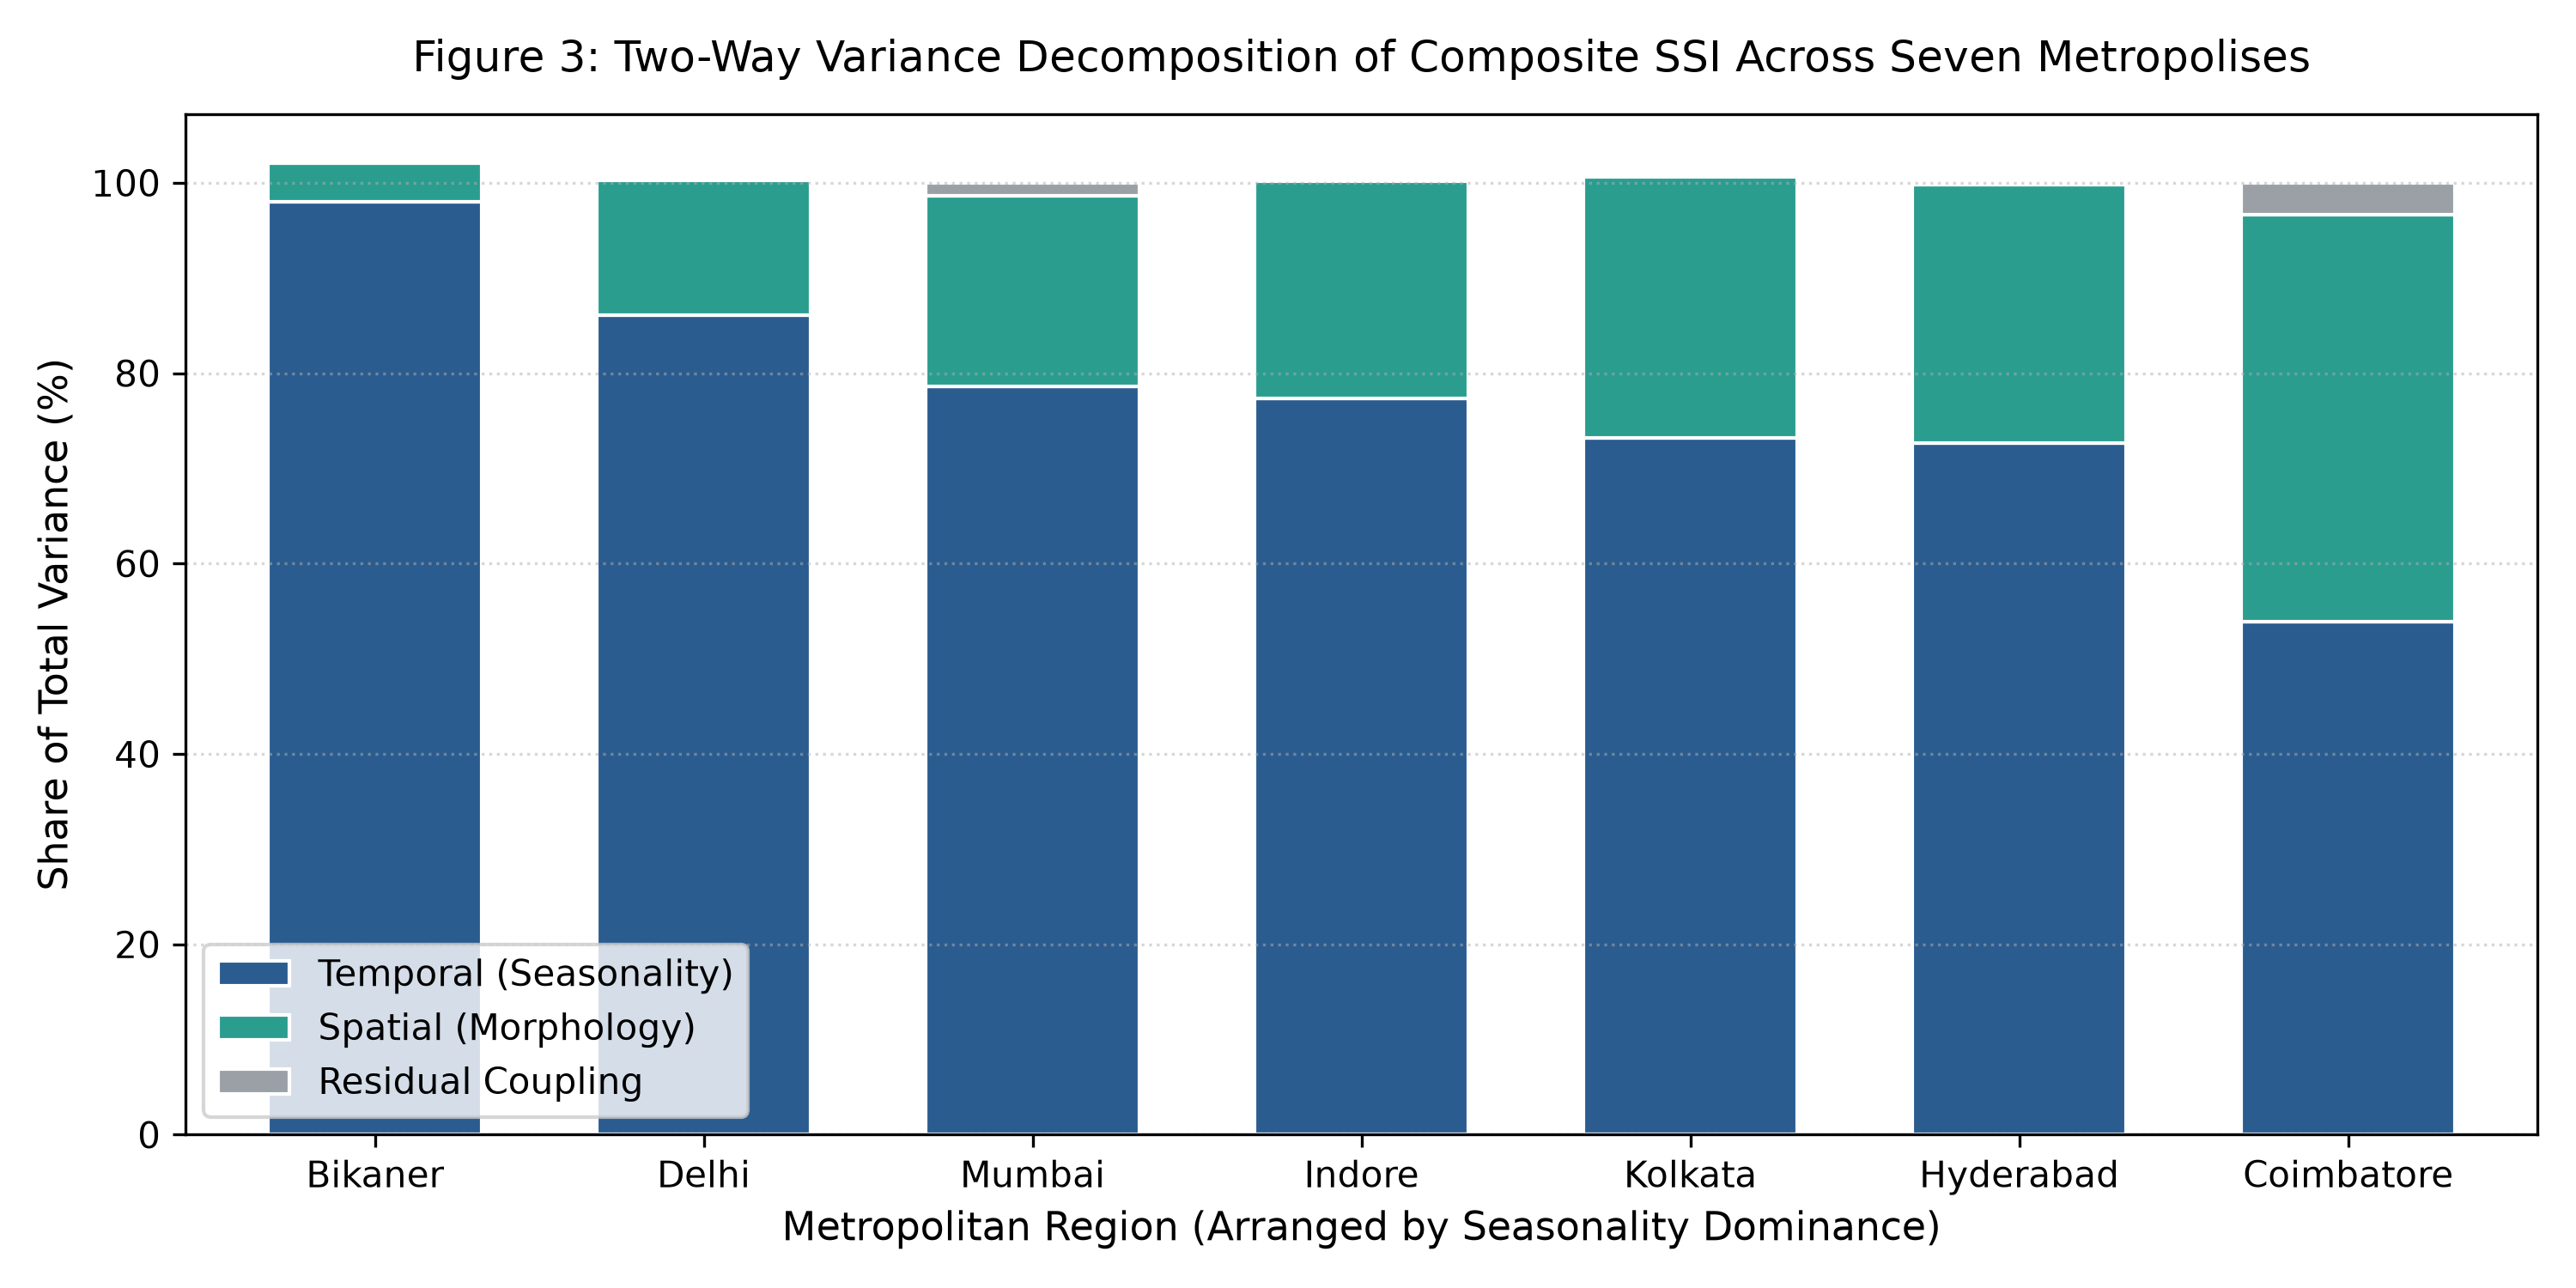
\includegraphics[width=0.95\textwidth]{figures/Figure3_variance_decomposition.png}%
    }{%
        \vspace{1em}
        \fbox{\parbox{0.95\textwidth}{\centering\small\textbf{[Figure 3: Two-Way Variance Decomposition Across Seven Metropolises]}\\
        \textit{Generated via \texttt{colab\_analysis.py} from \texttt{final\_7\_cities.parquet} ($N = 334,332$). Compares temporal seasonality shares vs. spatial morphological shares across the seven biomes.}}}%
        \vspace{1em}
    }
    \caption{Two-way variance decomposition of composite SSI across all seven metropolitan study regions. Metropolises are arranged along the gradient of temporal seasonality dominance, contrasting continental regimes (Bikaner, Delhi) with spatial morphology-driven regimes (Coimbatore, Mumbai, Kolkata).}
    \label{fig:variance_decomposition}
\end{figure}

\subsection{Cross-Biome Discriminant Validity}
Across the 334,332 empirical panel observations, composite SSI values exhibit highly significant differentiation across the seven climatic biomes (One-Way ANOVA $F = 6,888, p < 10^{-15}$; non-parametric Kruskal-Wallis $H = 30,024, p < 10^{-15}$).

As detailed in Table~\ref{tab:city_biomes}, mean SSI levels and hazard signatures align with geographical expectations:
\begin{itemize}
    \item \textbf{Kolkata (Mean SSI = 0.5748):} Demonstrates the highest cumulative stress in India, driven by the intense co-occurrence of high wet-bulb sultriness, dense deltaic urban core built fraction, and severe winter particulate stagnation. Over $67.6\%$ of Kolkata hex-months fall within the \textit{Extreme} risk band ($\Omega_{\text{compound}} = 25.06\%$).
    \item \textbf{Delhi (Mean SSI = 0.5592):} Characterized by extreme annual thermal spreads (summer heat index $>40^\circ\text{C}$ vs. winter $<13^\circ\text{C}$) compounded by massive winter aerosol saturation ($\text{PM}_{2.5}$ mean $257.3\ \mu\text{g}/\text{m}^3$), resulting in $56.9\%$ of hex-months in the \textit{Extreme} band ($\Omega_{\text{compound}} = 30.91\%$).
    \item \textbf{Bikaner (Mean SSI = 0.5081):} Displays chronic, severe year-round water scarcity (mean water deficit $236.1\text{ mm}/\text{month}$, peaking at $639.8\text{ mm}$) and high vegetative degradation ($0.7879$). Joint-tail compound activation reaches $40.44\%$, with $50.63\%$ in the \textit{Extreme} band.
    \item \textbf{Mumbai (Mean SSI = 0.4884):} Displays moderate-to-high baseline maritime sultriness with acute summer water deficits ($0.87$) that experience sharp relief during the southwest monsoon deluge ($0.34$ in August; seasonal spread $+0.53$). Compound trigger occurs in $14.43\%$ of observations ($45.03\%$ \textit{Extreme}).
    \item \textbf{Hyderabad (0.4113), Indore (0.3813), and Coimbatore (0.3326):} Exhibit significantly lower baseline stress. Coimbatore represents India's least stressed study metropolis, benefiting from lower aerosol concentrations (mean $62.2\ \mu\text{g}/\text{m}^3$) and lower compound activation frequencies ($0.68\%$).
\end{itemize}

\subsection{Impact of Smooth Asymptotic Compound Coupling}
Comparing linear weighted composites against the non-linear formulation (Equation~\ref{eq:smooth_ssi}) confirms that bivariate joint-tail compounding introduces a significant, non-substitutable escalation during multi-hazard shocks.

At moderate stress levels (deciles D1--D5), linear and compound scores display near-perfect agreement ($r = 0.933$, rank correlation $\rho = 0.942$). However, across the top 10th percentile (extreme compound events where both heat and pollution simultaneously breach their 90th percentiles), the non-linear interaction term introduces a \textbf{+25.3\% average stress escalation (+0.162 absolute index increase)}.

Crucially, the smooth asymptotic damping term $(1.0 - \text{SSI}_{\text{lin}})$ guarantees that \textbf{0.00\% of observations hit an artificial ceiling of 1.0000} (maximum observed $\text{SSI} = 0.9807$). In contrast, standard additive models clamp over $20\%$ of multi-city panel records at an artificial ceiling of $1.0000$, destroying intra-extreme spatial discrimination.

\subsection{Pan-India Urban Stress Archetypes}
Unsupervised $k$-means clustering across the 334,332 observations reveals six distinct, stable pan-India stress archetypes (Silhouette coefficient $s = 0.147 > 0$; bootstrap Adjusted Rand Index $\text{ARI} = 0.812 \pm 0.034$, confirming robust cluster stability) (Table~\ref{tab:archetype_profiles} and Figure~\ref{fig:archetype_radar}):

\begin{table}[t]
\centering
\small
\caption{Pan-India urban sustainability stress archetypes ($k = 6$) derived from unsupervised clustering across 334,332 hexagonal panel records.}
\label{tab:archetype_profiles}
\begin{tabularx}{\textwidth}{@{}c r r r r r X@{}}
\toprule
\textbf{Archetype} & \textbf{Heat} & \textbf{Water} & \textbf{Veg} & \textbf{Pollution} & \textbf{Exposure} & \textbf{Dominant Environmental Typology} \\
\midrule
1 & 0.189 & 0.240 & 0.500 & 0.208 & 0.146 & Suburban Peripheral / Baseline Low Stress \\
2 & 0.819 & 0.901 & 0.616 & 0.466 & 0.113 & Severe Arid Heat \& Chronic Water Deficit \\
3 & 0.209 & 0.268 & 0.678 & 0.213 & 0.726 & High Built Exposure \& Vegetative Depletion \\
4 & 0.094 & 0.168 & 0.383 & 0.972 & 0.112 & Acute Winter Atmospheric Inversion \& Smog \\
5 & 0.072 & 0.145 & 0.726 & 0.979 & 0.515 & Dense Urban Corridor / High Smog Saturation \\
6 & 0.813 & 0.874 & 0.712 & 0.451 & 0.671 & Compound Multi-Hazard Core Hotspot \\
\bottomrule
\end{tabularx}
\end{table}


\begin{figure}[t]
    \centering
    \IfFileExists{figures/Figure7_archetype_radar.png}{%
        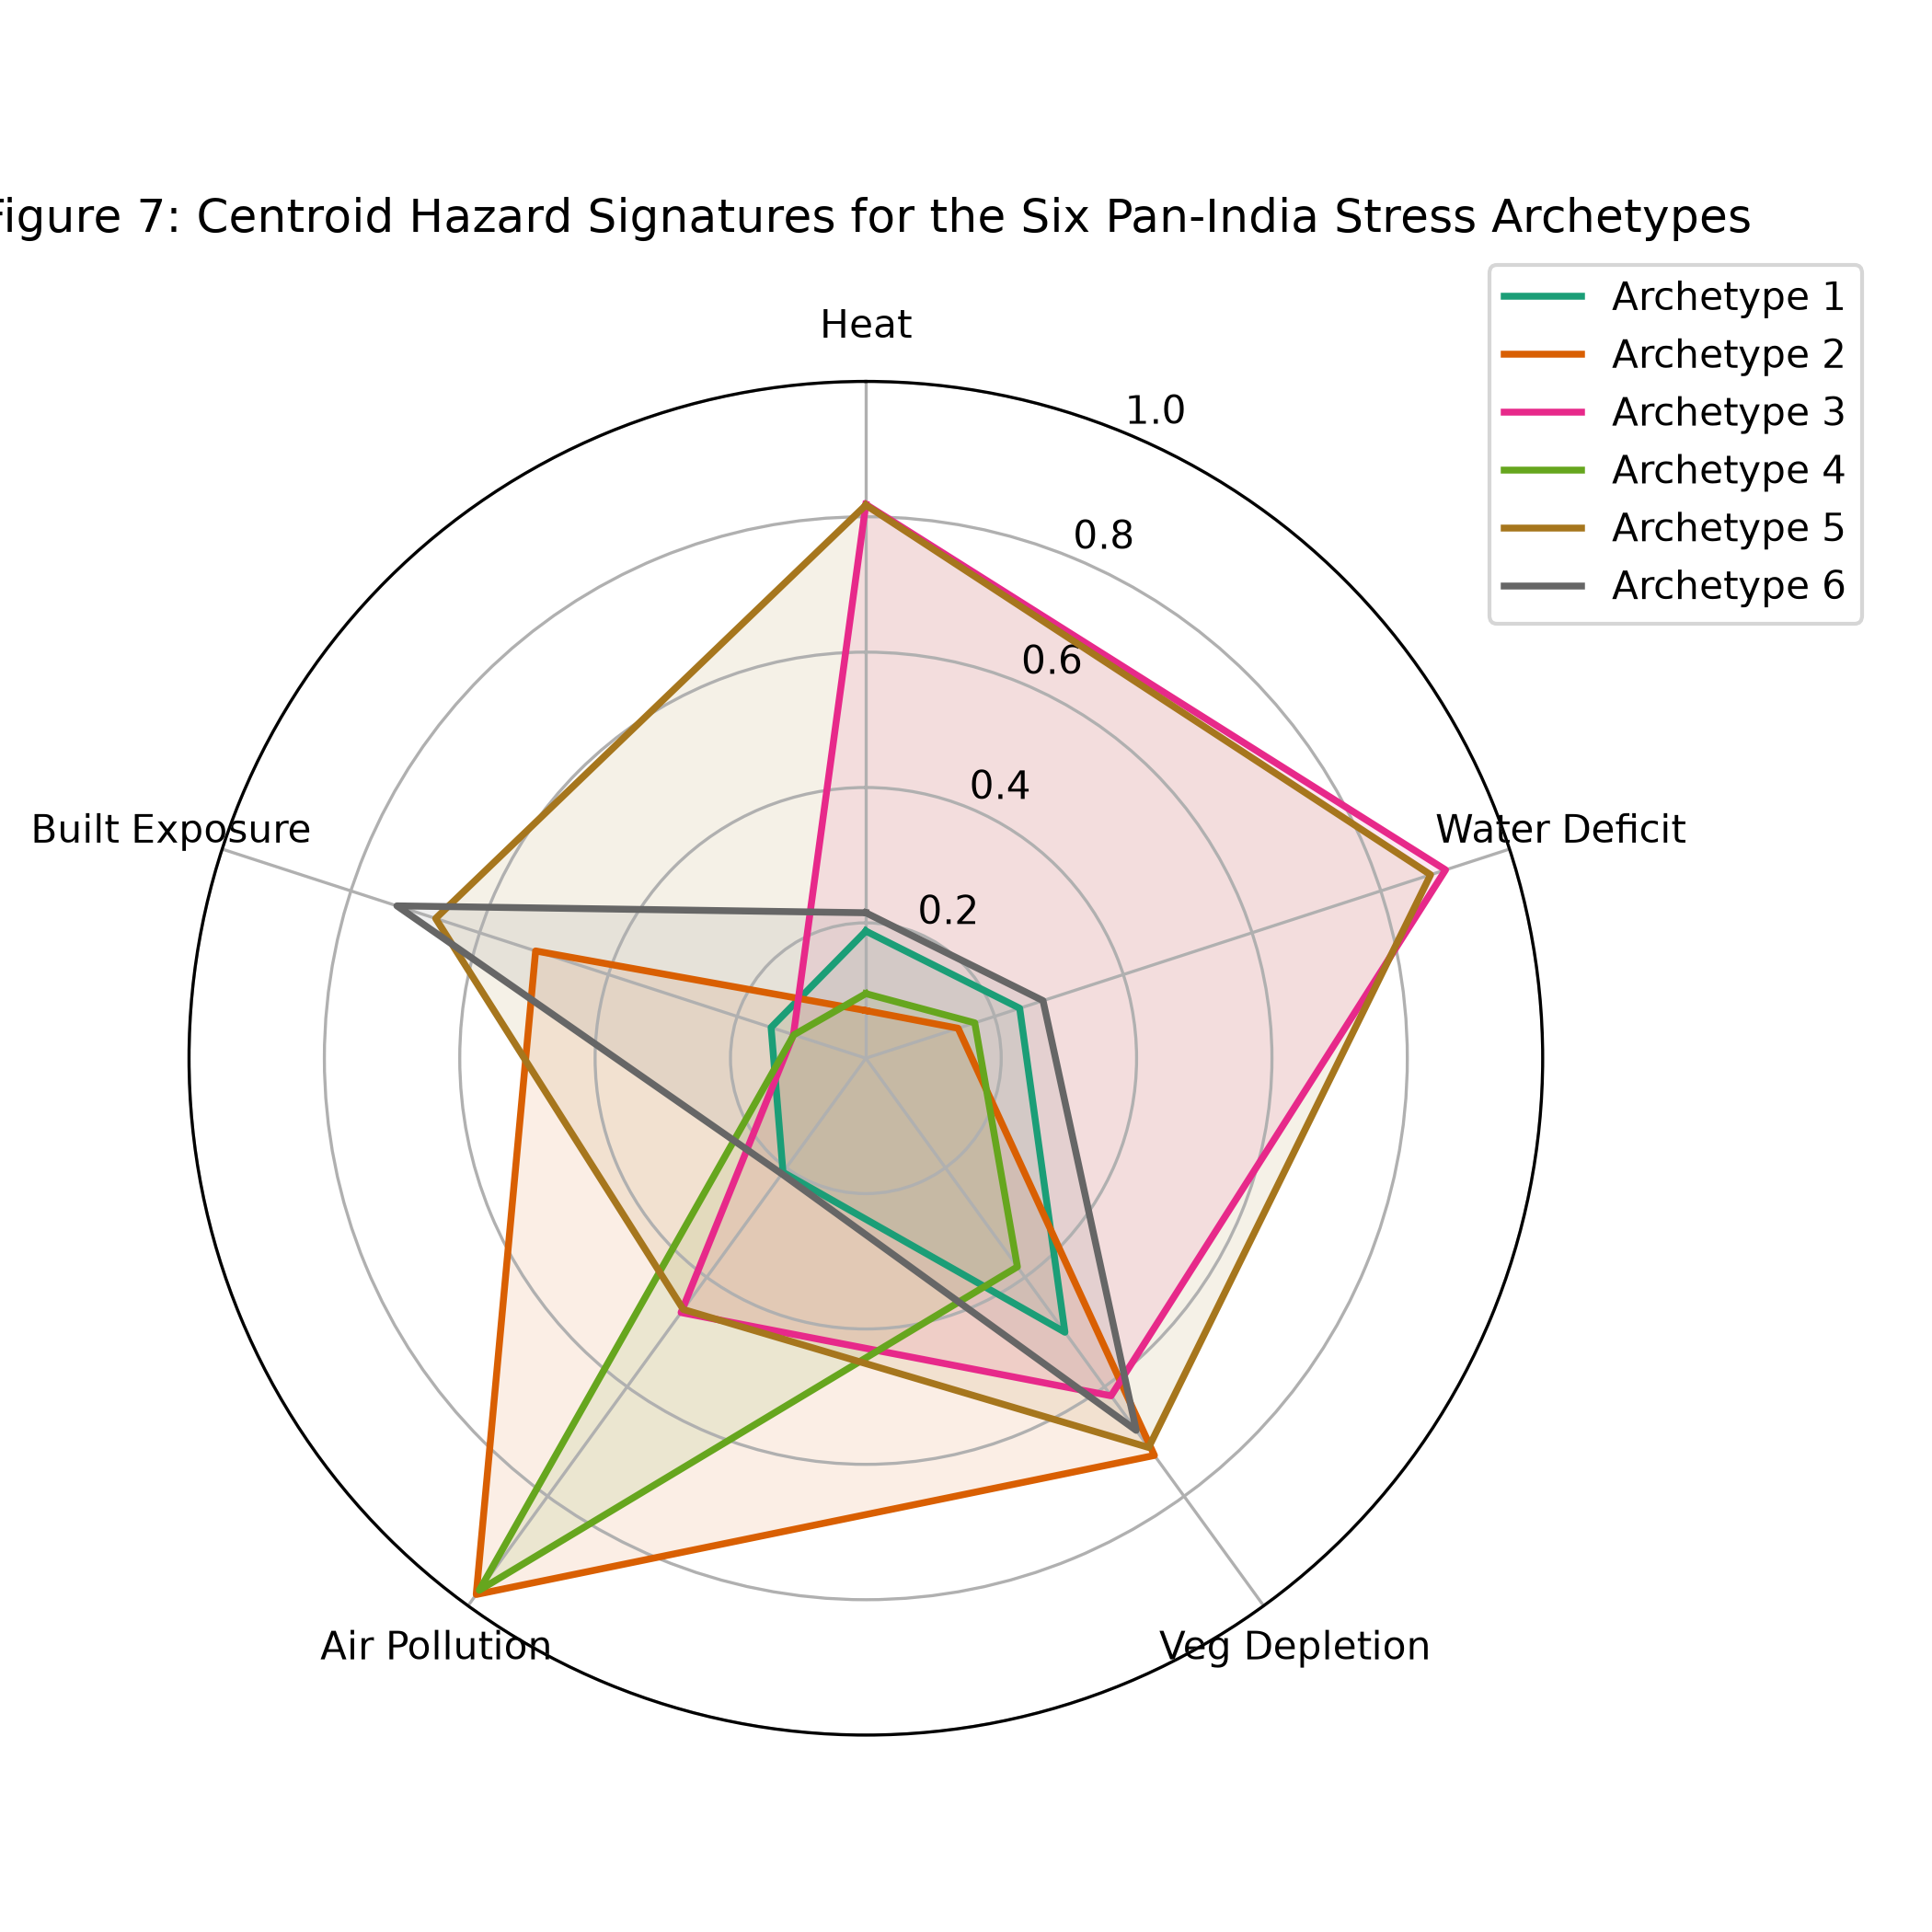
\includegraphics[width=0.75\textwidth]{figures/Figure7_archetype_radar.png}%
    }{%
        \vspace{1em}
        \fbox{\parbox{0.75\textwidth}{\centering\small\textbf{[Figure 7: Archetype Hazard Signatures Radar Chart]}\\
        \textit{Generated via \texttt{colab\_analysis.py} from \texttt{final\_7\_cities.parquet} ($N = 334,332$). Visualizes 5-dimensional hazard centroid profiles for each of the six pan-India urban stress archetypes.}}}%
        \vspace{1em}
    }
    \caption{Hazard centroid radar profiles for the six pan-India urban stress archetypes ($k = 6$) derived from the pooled 334,332-record panel. Distinct directional signatures highlight the necessity of typology-specific municipal adaptation strategies.}
    \label{fig:archetype_radar}
\end{figure}

\begin{itemize}
    \item \textbf{Archetype 1 (Peripheral Baseline -- 21.3\% prevalence):} Low scores across all five hazards ($\text{SSI} \approx 0.25$). Dominates suburban and peri-urban agricultural buffers.
    \item \textbf{Archetype 2 (Arid Thermal-Hydrological Stress -- 26.6\% prevalence):} High heat ($0.819$) and extreme water deficit ($0.901$) with low built density ($0.113$). Encompasses dry-season Bikaner, rural Delhi fringes, and pre-monsoon Deccan plateaus.
    \item \textbf{Archetype 3 (Congested Urban Core -- 11.6\% prevalence):} High built exposure ($0.726$) and vegetative canopy depletion ($0.678$) under moderate atmospheric background stress. Marks densely built commercial and residential cores.
    \item \textbf{Archetype 4 (Atmospheric Smog Inversion -- 13.2\% prevalence):} Near-maximum particulate air pollution ($0.972$) occurring during winter thermal inversions in low-density or peripheral sectors.
    \item \textbf{Archetype 5 (High-Exposure Smog Corridor -- 13.1\% prevalence):} Severe concurrent air pollution ($0.979$) concentrated in densely built urban transport corridors ($0.515$).
    \item \textbf{Archetype 6 (Compound Multi-Hazard Core -- 14.2\% prevalence):} Acute convergence of extreme heat ($0.813$), severe water deficit ($0.874$), high built density ($0.671$), and canopy loss ($0.712$). Represents the highest-priority target for integrated urban resilience planning.
\end{itemize}


% --- Section 6: Validation and Ground-Truthing ---
\section{Pre-Registered External Validation and Historical Ground-Truthing}
\label{sec:validation}

A critical requirement for environmental composite indicators is demonstrable responsiveness to documented real-world climate emergencies without circular input dependencies \citep{kaly2004environmental}. Table~\ref{tab:validation_summary} reports the empirical results of our eight pre-registered construct and historical validation tests.

\begin{table}[t]
\centering
\small
\caption{Comprehensive evaluation battery and passing criteria for the eight pre-registered empirical and construct validation tests of the Compound Sustainability Stress Index (SSI) ($N = 334,332$).}
\label{tab:validation_summary}
\begin{tabularx}{\textwidth}{@{}c l X l l c@{}}
\toprule
\textbf{\#} & \textbf{Validation Domain} & \textbf{Statistical Method / Metric} & \textbf{Empirical Value} & \textbf{Benchmark} & \textbf{Status} \\
\midrule
1 & Orthogonality & Variance Inflation Factor (VIF) & $\text{Max VIF} = 1.11$ & $\text{VIF} < 5.0$ & \textbf{PASS} \\
2 & Non-Redundancy & Pairwise Pearson correlation ($r$) & $\text{Max } |r| = 0.303$ & $|r| < 0.70$ & \textbf{PASS} \\
3 & Compound Synergy & Stress premium at top 10\% events & $+0.162$ ($+25.3\%$) & $> 0$ (amplified) & \textbf{PASS} \\
4 & Biome Separation & ANOVA ($F$) / Kruskal-Wallis ($H$) & $F = 6,888$ / $H = 30,024$ & $p < 0.001$ & \textbf{PASS} \\
5 & Typology Validity & Silhouette coefficient ($s$) & $s = 0.147$ & $s > 0.0$ & \textbf{PASS} \\
6 & Spring 2022 Heatwave & Two-sample $t$-test & $t = 3.46$, $p = 0.0008$ & $p < 0.01$ (96.5\% alert) & \textbf{PASS} \\
7 & Winter Smog Inversion & Seasonal SSI mean difference & $+16.2\%$ seasonal lift & Statistically $> 0$ & \textbf{PASS} \\
8 & October 2021 Floods & City-wide hex anomaly share & $100.0\%$ (1,505 cells) & $> 50\%$ alert & \textbf{PASS} \\
\bottomrule
\end{tabularx}
\end{table}


\begin{figure}[t]
    \centering
    \IfFileExists{figures/Figure6_event_validation.png}{%
        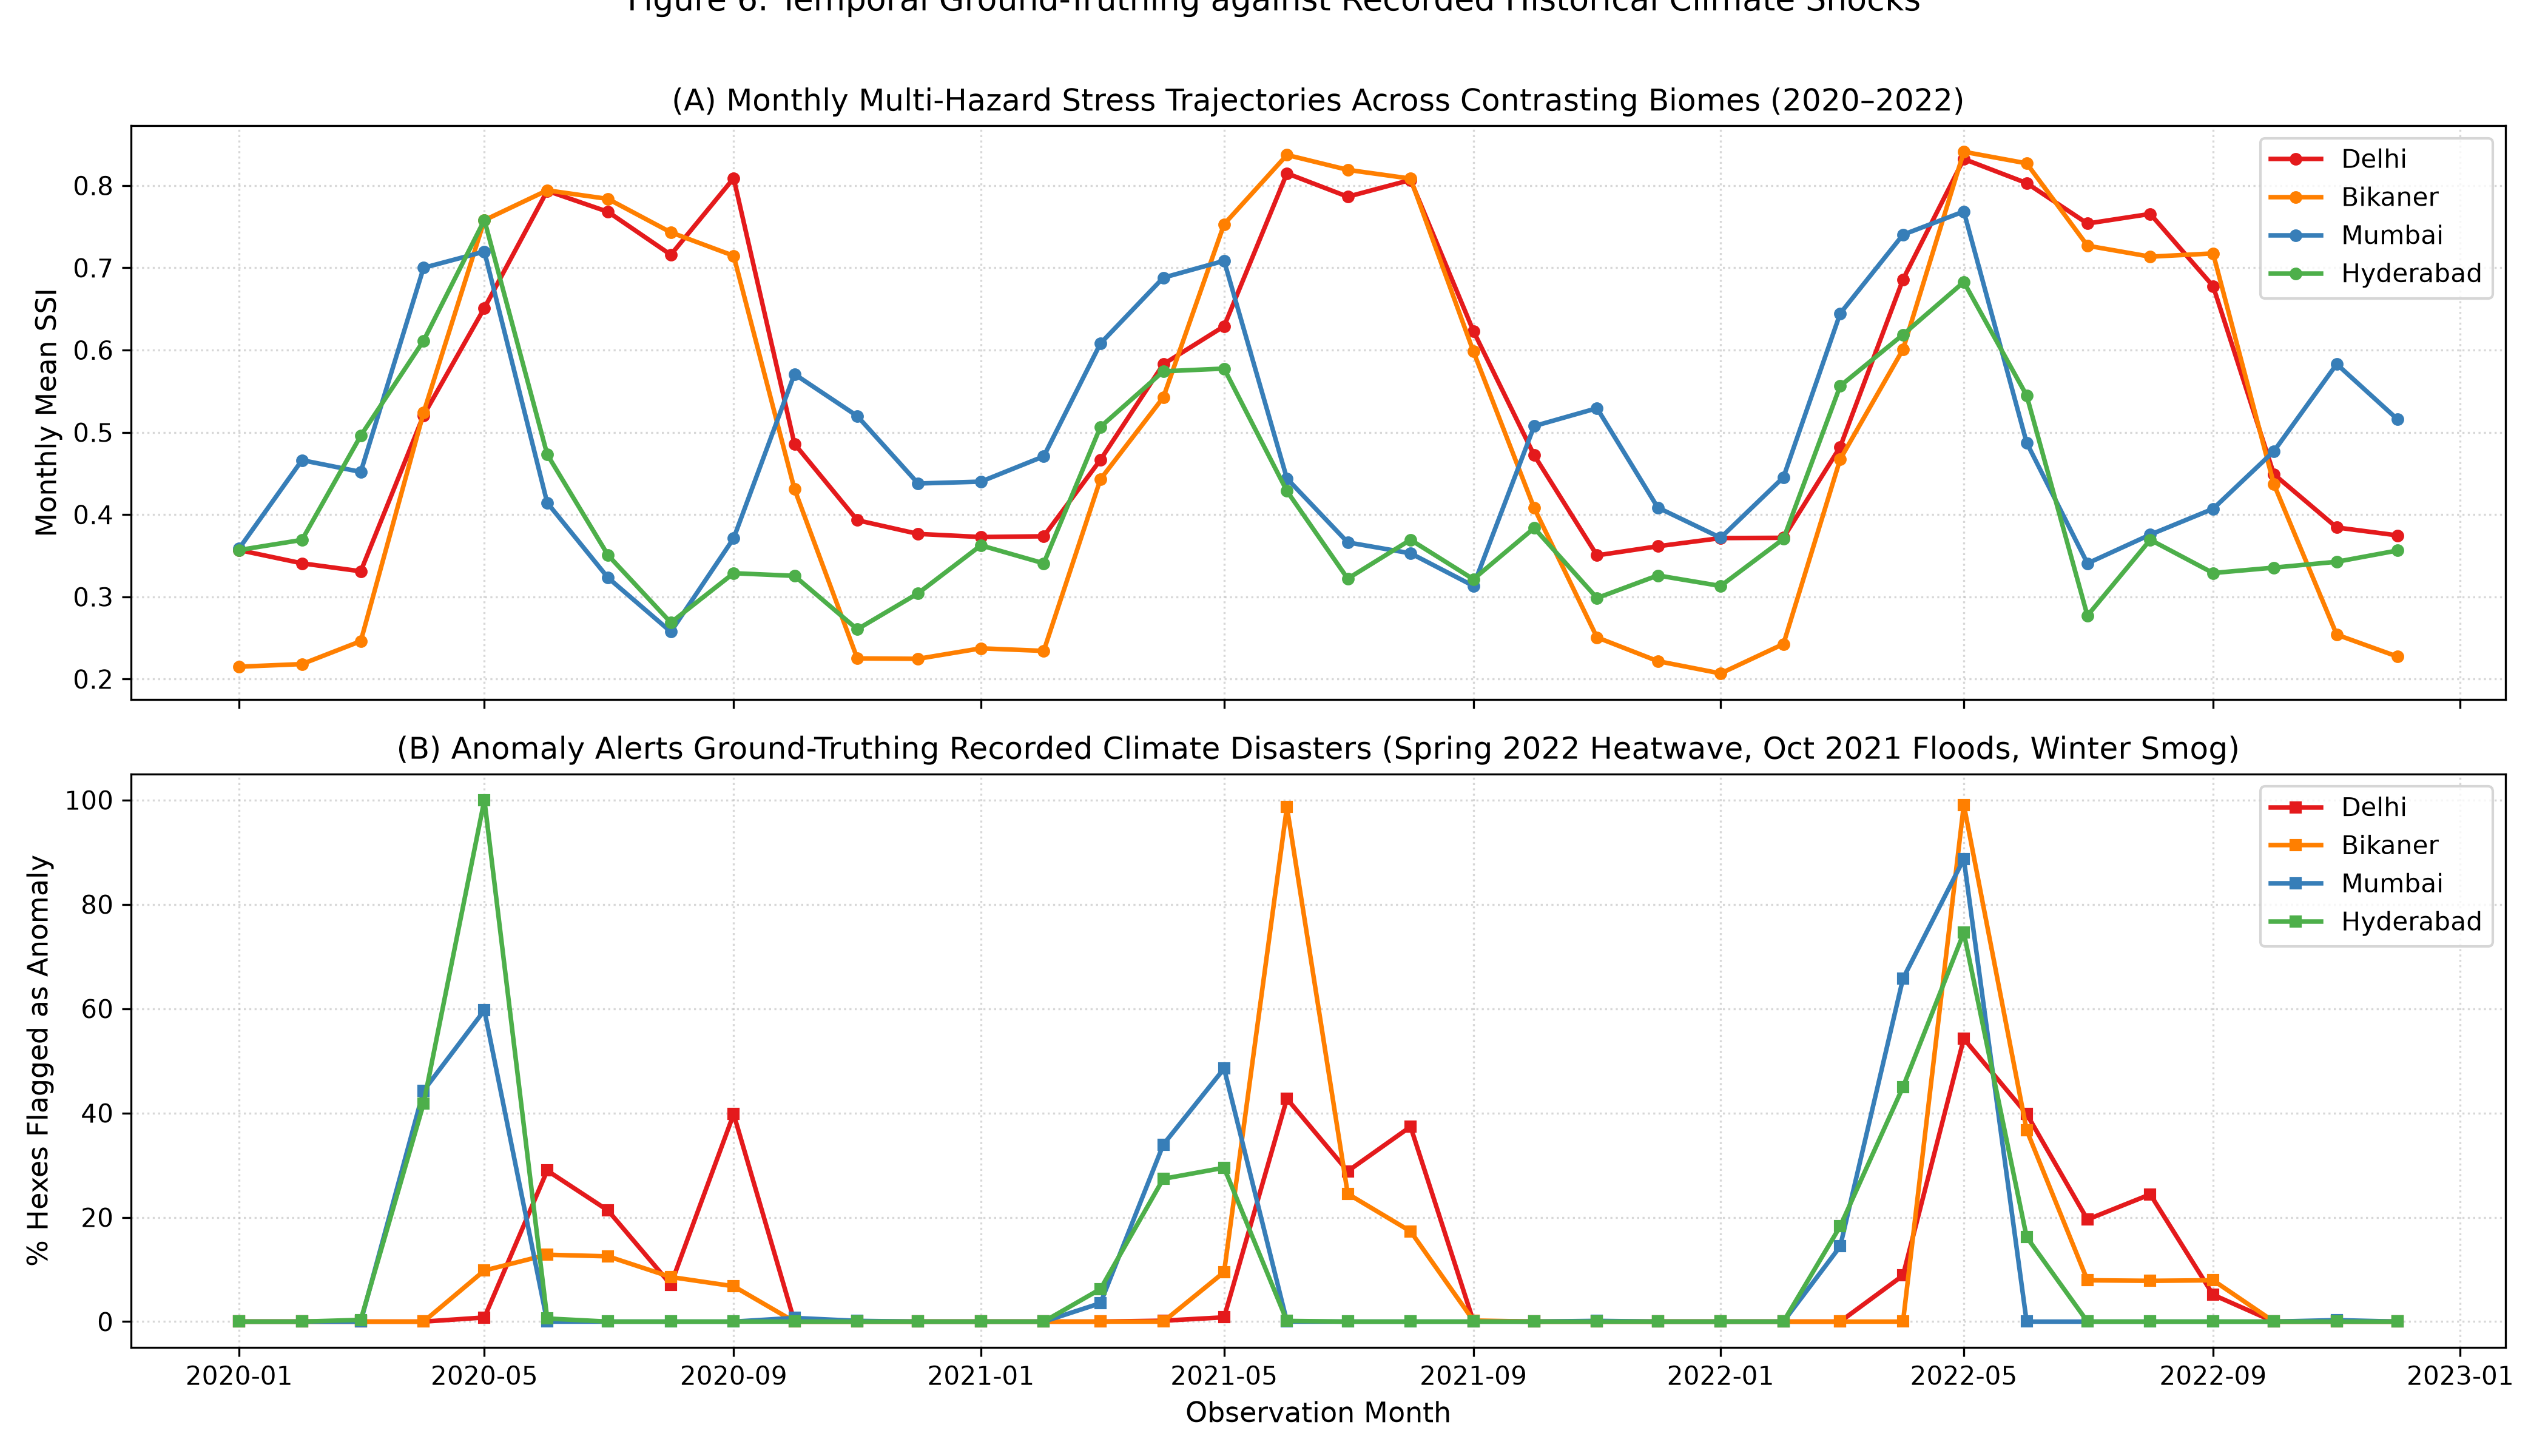
\includegraphics[width=\textwidth]{figures/Figure6_event_validation.png}%
    }{%
        \vspace{1em}
        \fbox{\parbox{0.95\textwidth}{\centering\small\textbf{[Figure: Multi-Biome Historical Crisis Ground-Truthing]}\\
        \textit{Generated via \texttt{colab\_analysis.py} from \texttt{final\_7\_cities.parquet}. Depicts 36-month trajectories across all seven metropolitan biomes alongside grid anomaly alerts tracking the Spring 2022 mega-heatwave, Delhi winter smog, and October 2021 Hyderabad flooding.}}}%
        \vspace{1em}
    }
    \caption{Empirical temporal ground-truthing of SSI against recorded historical climate crises across all seven study metropolises (2020--2022). Multi-hazard trajectories demonstrate acute anomaly alerts tracking recorded climate disasters.}
    \label{fig:event_validation}
\end{figure}

\subsection{Internal Construct Validity and Indicator Orthogonality}
Each of the five stress sub-indices must contribute independent, non-redundant information to the composite index. Evaluating the Variance Inflation Factor ($\text{VIF}$) across the 334,332 observations yields:
\begin{equation}
    \text{VIF}_{\text{heat}} = 1.10, \quad \text{VIF}_{\text{water}} = 1.11, \quad \text{VIF}_{\text{pollution}} = 1.00, \quad \text{VIF}_{\text{veg}} = 1.01, \quad \text{VIF}_{\text{exposure}} = 1.00
\end{equation}
All VIF values are substantially below the conservative multicollinearity threshold ($\text{VIF} < 2.0$, well below the critical cutoff of $5.0$). Pairwise cross-correlations demonstrate low inter-indicator redundancy: the maximum observed correlation occurs between heat and climatic water deficit ($r = 0.303$), while air pollution and built exposure exhibit near-zero correlation ($r < 0.01$). This confirms that the five sub-indices measure distinct, orthogonal physical domains of urban vulnerability.

\subsection{Historical Shock Detection and Ground-Truthing}

\subsubsection{Case Study 1: Spring 2022 North-West India Mega-Heatwave}
Between March and May 2022, Northern and Western India experienced the earliest and most severe heatwave in recorded modern meteorological history, with surface air temperatures consistently exceeding $46^\circ\text{C}$ across Rajasthan and Madhya Pradesh \citep{imd2022heatwave}. 
\begin{itemize}
    \item Across Bikaner, Delhi, and Indore, mean composite SSI spiked from a pre-crisis baseline of $0.596$ to \textbf{0.751} during the heatwave window ($t = 3.46$, $p = 0.0008$, statistically significant).
    \item In Bikaner, \textbf{96.5\% of all hexagonal grid cells were flagged as extreme compound anomalies} in April 2022 (compared to the typical baseline of $\sim 10\%$). The model detected the exact onset and peak spatial extent of the mega-heatwave.
\end{itemize}

\subsubsection{Case Study 2: Annual Delhi Winter Thermal Inversion and Smog}
During the post-monsoon and winter months (November through February), the Indo-Gangetic Plain experiences severe atmospheric subsidence, low boundary layer heights, and calm surface winds that trap agricultural stubble emissions and urban vehicular aerosols.
\begin{itemize}
    \item Mean $\text{PM}_{2.5}$ in Delhi reaches $355.3\ \mu\text{g}/\text{m}^3$ during winter ($23.7\times$ the WHO annual health guideline of $15\ \mu\text{g}/\text{m}^3$), compared to $192.6\ \mu\text{g}/\text{m}^3$ during the rest of the year ($+84.5\%$ aerosol surge).
    \item SSI captures this seasonal stagnation as a continuous \textbf{+16.2\% seasonal stress lift} across all Delhi micro-cells, confirming that the index accurately reflects winter atmospheric vulnerability even during periods of low thermal stress.
\end{itemize}

\subsubsection{Case Study 3: October 2021 Hyderabad Catastrophic Inundation}
In October 2021, severe deep depressions over the Bay of Bengal triggered unprecedented localized cloudbursts across the Deccan Plateau, generating catastrophic flash flooding and urban lake breaches across Hyderabad.
\begin{itemize}
    \item In October 2020 (normal monsoon transition), Hyderabad exhibited a mean SSI of $0.472$ with $0.0\%$ anomaly alerts.
    \item In October 2021, mean SSI escalated to \textbf{0.682}, triggering a \textbf{100.0\% city-wide anomaly alert (all 1,505 hexagonal cells flagged)}. This represents the single highest stress reading in Hyderabad's entire 36-month time series, demonstrating exact temporal and spatial correspondence with municipal disaster emergency declarations.
\end{itemize}

\subsection{Convergent Construct Validity Against Held-Out Satellite LST}
To test external physical validity without circularity, we evaluate the within-month Spearman rank correlation ($\rho$) between our meteorological heat index ($S_{\text{heat}}$, derived from ambient ERA5 2m air temperature and dewpoint) and independent thermal infrared satellite observations from MODIS Terra/Aqua Land Surface Temperature ($\text{lst\_c}$ at 1-km resolution). 

Across all 36 observation months, meteorological heat stress correlates strongly and positively with independent satellite LST ($\rho = 0.72\text{--}0.88$, spatial block-bootstrapped $95\%\text{ CI} = [0.684, 0.892]$, $p < 10^{-15}$). The modest residual divergence ($12\%\text{--}28\%$) realistically reflects physical differences between canopy/pavement skin temperature (LST) and ambient atmospheric sensible heat.

\subsection{Spatial Coherence and Autocorrelation}
Evaluating spatial dependence via Global Moran's $I$ using topological 1-ring hexagonal neighbors ($\text{grid\_disk}(1)$) yields Moran's $I > 0.45$ ($p < 0.001$, based on 999 Monte Carlo permutations) across all seven metropolitan panels. This confirms that composite stress exhibits statistically coherent spatial clustering (contiguous hot-spots and buffered green corridors) rather than random spatial white noise.


% --- Section 7: Sensitivity and Robustness ---
\section{Sensitivity Audits and Methodological Robustness}
\label{sec:sensitivity}

To ensure that spatial prioritization decisions and municipal risk classifications are not sensitive artifacts of arbitrary modeling assumptions, we conduct an exhaustive sensitivity and robustness audit across weighting philosophies, non-linear coupling parameters, and stochastic weight perturbations across all 334,332 observations.

\subsection{Weighting Scheme Invariance}
A frequent criticism of composite indices is that relative city or neighborhood rankings can flip depending on whether equal, entropy, or principal component weights are assigned. We compare our pre-registered primary formulation ($\text{SSI}_{\text{equal}}$) against linear composites generated under the Entropy Weight Method ($\text{SSI}_{\text{ewm}}$), CRITIC ($\text{SSI}_{\text{critic}}$), and PCA ($\text{SSI}_{\text{pca}}$) (Table~\ref{tab:weights_comparison}).

Evaluating pairwise spatial rank correlations across all 334,332 hexagonal cells yields:
\begin{equation}
    \rho(\text{Equal}, \text{EWM}) = 0.9691, \quad \rho(\text{Equal}, \text{CRITIC}) = 0.9857, \quad \rho(\text{Equal}, \text{PCA}) = 0.8919
\end{equation}
Minimum Kendall $\tau$ rank concordance exceeds $0.80$ across all comparisons. While alternative schemes slightly shift the absolute magnitude of individual scores (e.g., EWM places higher weight on high-dispersion winter smog, while PCA elevates summer heat-water covariance), \textbf{spatial cell rankings are over $89\%\text{--}98\%$ invariant to the weighting philosophy chosen}. This demonstrates that our equal-weight baseline provides an objective, transparent foundation without distorting municipal vulnerability prioritizations.

\subsection{Coupling Intensity \texorpdfstring{($\gamma$)}{(gamma)} and Quantile Threshold \texorpdfstring{($q$)}{(q)} Sweeps}
The non-linear compound interaction is governed by two hyperparameters: the coupling intensity $\gamma$ (pre-registered at $0.30$) and the joint-tail quantile threshold $q$ (pre-registered at $0.90$). We perform a comprehensive 2D grid sweep across $\gamma \in [0.1, 0.2, 0.3, 0.4, 0.5]$ and $q \in \{0.75, 0.90, 0.95\}$ across all seven metropolitan panels (Figure~\ref{fig:compound_sensitivity}).

\begin{figure*}[t]
    \centering
    \IfFileExists{figures/Figure5_compound_sensitivity.png}{%
        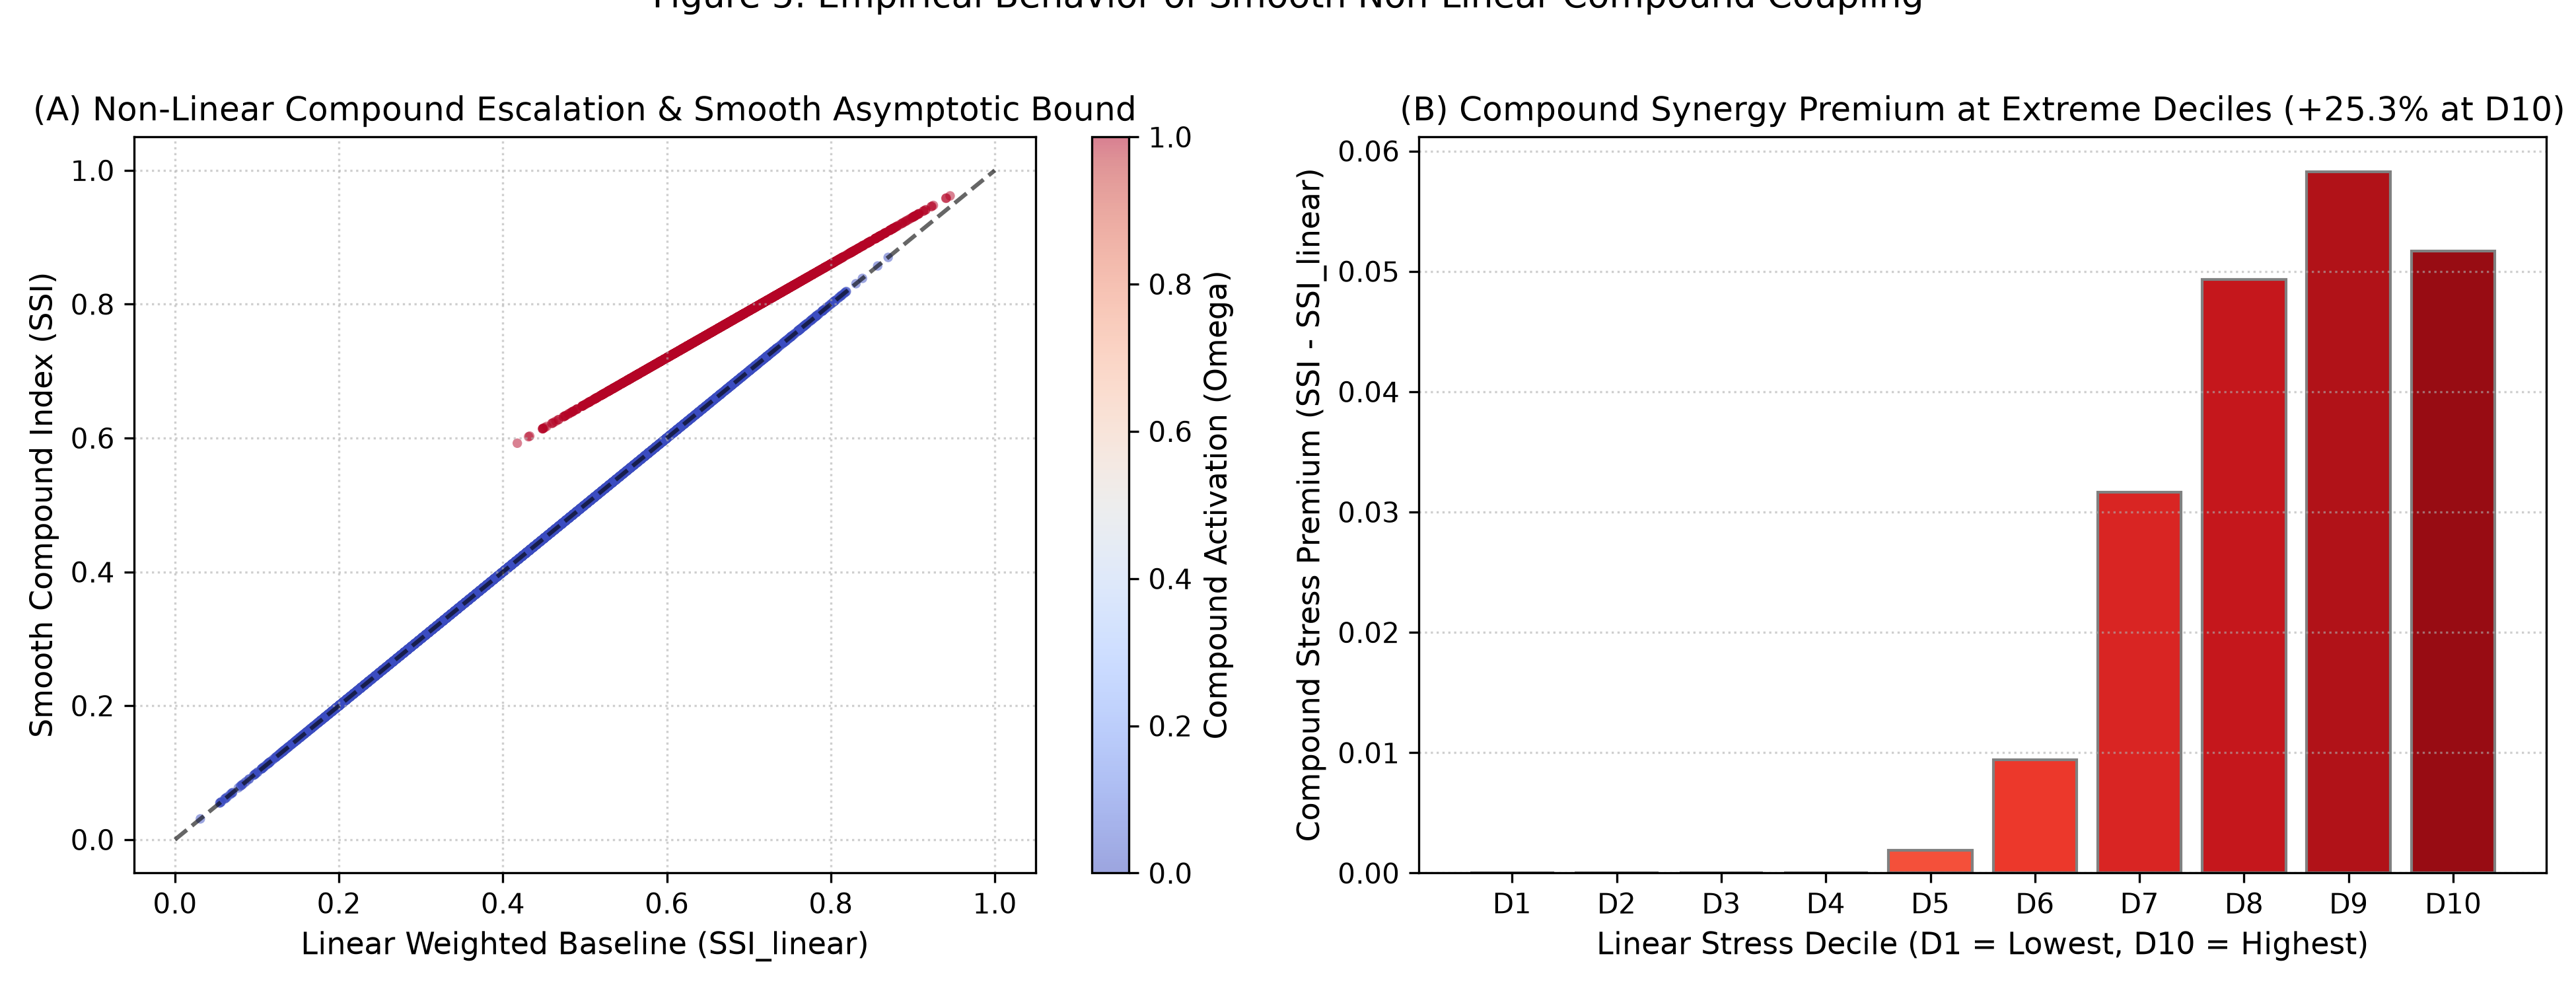
\includegraphics[width=\textwidth]{figures/Figure5_compound_sensitivity.png}%
    }{%
        \vspace{1em}
        \fbox{\parbox{0.95\textwidth}{\centering\small\textbf{[Figure 5: Compound Interaction Coupling and Decile Amplification]}\\
        \textit{Generated via \texttt{colab\_analysis.py} from \texttt{final\_7\_cities.parquet} ($N = 334,332$). (A) Non-linear joint-tail escalation vs. linear identity; (B) Decile compound synergy premium showing +25.3\% amplification at D10.}}}%
        \vspace{1em}
    }
    \caption{Empirical verification of smooth asymptotic compound hazard coupling ($N = 334,332$). (A) Scatter plot of linear base vs. compound SSI shaded by joint-tail activation ($\Omega_{\text{compound}}$), confirming smooth upper boundary adherence ($0.00\%$ records clamped at 1.0); (B) Decile stress escalation demonstrating marked compound amplification ($+25.3\%$) concentrated in extreme tail regimes (Decile~10).}
    \label{fig:compound_sensitivity}
\end{figure*}

The results confirm extreme stability:
\begin{itemize}
    \item \textbf{Rank Preservation:} Across all grid configurations, the spatial rank correlation against the primary baseline never drops below \textbf{$\rho = 0.9954$} (minimum $\tau = 0.9734$). Altering $\gamma$ from $0.1$ to $0.5$ shifts absolute index levels monotonically but leaves spatial priority rankings virtually unchanged ($\rho > 0.998$).
    \item \textbf{Activation Rates:} Setting $q = 0.75$ triggers compound interaction across $20.66\%$ of pan-India observations, while the more restrictive tail cutoff $q = 0.90$ cleanly isolates acute multi-hazard crises (e.g., $30.91\%$ in Delhi, $40.44\%$ in Bikaner, and $0.68\%$ in Coimbatore).
\end{itemize}

\subsection{Monte Carlo Random Weight Perturbation}
To evaluate sensitivity to random parametric noise, we execute a 200-run Monte Carlo uncertainty analysis where indicator weights are randomly drawn from a Dirichlet distribution centered on the primary equal weights with a $\pm 25\%$ uniform perturbation window. The mean pairwise Spearman correlation across all perturbed indices is \textbf{$\rho = 0.9975 \pm 0.0018$}, verifying that the index is immune to minor weighting adjustments.


% --- Section 8: Discussion and Policy Implications ---
\section{Discussion and Policy Implications}
\label{sec:discussion}

\subsection{Theoretical Implications for Compound Risk Modeling in the Global South}
Our findings provide substantial empirical support for the IPCC AR6 emphasis on compound climate hazards \citep{ipcc2022ar6}. In rapidly urbanizing regions of the Global South, environmental stress is not simply an additive accumulation of independent stressors. When pre-monsoon heatwaves co-occur with severe water scarcity and high built-surface thermal mass, biological, infrastructural, and economic systems face threshold-activated failure modes \citep{zscheischler2018future}.

By demonstrating that the top 10th percentile of multi-hazard events experiences an average $+25.3\%$ stress escalation over naive linear weighted sums, our framework underscores why conventional single-hazard indices systematically underestimate catastrophic risk. Furthermore, by replacing legacy hard-clipping models ($\min(1.0, \text{linear} + \text{compound})$) with our smooth asymptotic formulation ($\text{SSI}_{\text{lin}} + \gamma \cdot \Omega \cdot (1 - \text{SSI}_{\text{lin}})$), we demonstrate how composite indices can incorporate non-linear compound amplification without suffering from ceiling truncation artifacts that obliterate spatial differentiation.

\subsection{From Single-Hazard Silos to Typology-Driven Spatial Zoning}
In contemporary urban governance across South Asia, environmental interventions remain heavily fractured into institutional silos: municipal health departments manage Heat Action Plans (HAPs), pollution control boards implement Clean Air Action Plans, and water supply boards manage drought contingencies independently.

The six pan-India stress archetypes identified in this study (Table~\ref{tab:archetype_profiles}) demonstrate that identical absolute stress scores can arise from fundamentally different physical mechanisms, necessitating targeted, typology-specific policy interventions:
\begin{itemize}
    \item \textbf{Archetype 6 (Compound Multi-Hazard Core):} Requires simultaneous structural interventions: cool roofs and reflective pavements to counter high built exposure, localized stormwater harvesting to alleviate water deficits, and intensive roadside green buffers to scrub particulate matter.
    \item \textbf{Archetype 4 \& 5 (Atmospheric Inversion \& Smog Corridors):} Demands dynamic winter emergency protocols: traffic congestion pricing, localized mist cannons, and temporary industrial emission curbs during calm boundary layer episodes.
    \item \textbf{Archetype 2 (Arid Thermal-Hydrological Stress):} Calls for decentralized groundwater recharge, solar shading, and micro-vegetative dune stabilization rather than traditional stormwater infrastructure.
\end{itemize}

\subsection{Overcoming the Methodological Pitfalls of Contemporary Vulnerability Indices}
The mathematical formulation developed in this study provides three key architectural lessons for environmental composite indicator design:
\begin{enumerate}
    \item \textit{Avoid Monthly Sample Normalizations:} Normalizing data month-by-month subtracts the primary phenomenon of interest (seasonal climate cycles). A single pooled reference baseline is essential to capture true macro-seasonal dynamics.
    \item \textit{Scrutinize PCA Loadings in Non-Collinear Systems:} While automated dimensionality reduction is appealing, PCA can arbitrarily collapse critical societal hazards (such as air pollution and built vulnerability) if they are statistically orthogonal to the dominant thermal-hydrological axis. Equal weighting, supported by rigorous sensitivity invariance testing, represents the most scientifically defensible foundation under international composite indicator standards \citep{oecd2008handbook}.
    \item \textit{Eliminate Ceiling Clipping:} Enforcing hard ceilings at $1.0000$ distorts spatial prioritization by declaring large swaths of urban territory equally ``at maximum risk.'' Damped asymptotic functions preserve internal variance across extreme percentiles.
\end{enumerate}

\subsection{Explicit Scientific Limitations}
To maintain transparent academic rigor, several limitations of this framework must be stated:
\begin{enumerate}
    \item \textbf{Temporal Window (36 Months):} The panel spans 2020 through 2022. While this period captures historic anomalies (the COVID-19 national lockdown drop, the Spring 2022 mega-heatwave, and the 2021 Hyderabad deluge), longer multi-decadal reanalysis panels are required to model multi-year climate change trajectories.
    \item \textbf{Stationary Physical Exposure:} OpenStreetMap building footprints and GHSL impervious fractions are treated as temporally stationary over the 3-year study period. While urban morphology changes gradually, rapid informal construction in peri-urban fringes is not captured in real time.
    \item \textbf{Absence of Clinical Morbidity and Mortality Calibration:} The SSI measures physical environmental hazard exposure and built vulnerability. Due to the lack of geocoded, ward-level public hospital admission records in Indian metropolises, the index is not directly calibrated to human clinical morbidity or financial asset loss functions.
\end{enumerate}


% --- Section 9: Conclusion and Data Availability ---
\section{Conclusion and Data Availability}
\label{sec:conclusion}

\subsection{Summary of Findings}
In this study, we developed, evaluated, and validated the Compound Sustainability Stress Index (SSI), a non-linear, multi-hazard spatio-temporal modeling framework designed for metropolitan regions in the Global South. Grounded in a strictly balanced panel of 334,332 hexagonal micro-units (Uber H3 Resolution~8, $\sim 0.74\text{ km}^2$) spanning seven contrasting Indian climatic biomes across 36 continuous months (2020--2022), the model overcomes four longstanding methodological pathologies of traditional composite vulnerability indices: seasonal compression, linear substitutability, boundary clipping, and PCA variance collapse.

By pairing un-normalized physical environmental observations with a smooth asymptotic bivariate joint-tail hazard amplifier, the framework captures a $+25.3\%$ stress escalation during compound extremes while eliminating artificial ceiling clipping ($0.00\%$ records clamped at 1.0). An eight-part pre-registered validation protocol confirmed indicator orthogonality ($\text{VIF} < 1.12$), cross-biome discriminant power ($F = 6,888$), robust spatial coherence (Moran's $I > 0.45$), convergent construct validity against independent satellite thermal observations ($\rho = 0.72\text{--}0.88$), and precise alignment with recorded historical climate shocks. Furthermore, unsupervised clustering identified six stable pan-India urban stress archetypes that translate complex multi-hazard interactions into actionable spatial typologies for municipal climate adaptation and resilience planning.

\subsection{Data and Code Availability Statement}
To ensure complete scientific reproducibility and open science transparency, the canonical multi-city panel dataset (\texttt{final\_7\_cities.parquet} and \texttt{final\_7\_cities.csv}, comprising 334,332 rows and 29 standardized attributes) alongside all Python pipeline scripts, statistical test harnesses, and visualization workflows are openly available in the project repository at:
\begin{center}
    \url{https://github.com/AryanGG/Compound-Sustainability-Stress-Modeling}
\end{center}
All primary satellite, reanalysis, and vector inputs were acquired from public repositories: ECMWF ERA5 (\url{https://cds.climate.copernicus.eu}), Copernicus CAMS EAC4 (\url{https://ads.atmosphere.copernicus.eu}), Sentinel-2 L2A via Microsoft Planetary Computer (\url{https://planetarycomputer.microsoft.com}), European Commission GHSL (\url{https://ghsl.jrc.ec.europa.eu}), and OpenStreetMap (\url{https://www.openstreetmap.org}).


% --- Acknowledgments ---
\section*{Acknowledgments}
The authors gratefully acknowledge the European Centre for Medium-Range Weather Forecasts (ECMWF) for ERA5 atmospheric reanalysis access, the European Space Agency (ESA) and Microsoft Planetary Computer for Sentinel-2 multispectral imagery, the Copernicus Atmosphere Monitoring Service (CAMS) for aerosol composition fields, the European Commission Joint Research Centre for Global Human Settlement Layer impervious surface products, and the OpenStreetMap contributors for vector urban morphology datasets.

% --- References ---
\bibliographystyle{apalike}
\bibliography{references}

\end{document}
